\newpage
%\chapter{Hipótese}
 %   A hipótese deste trabalho é apresentar como o Instituto Federal de Goiás pode agregar com uma solução de pesquisa, que tem como proposta construir um Sistema de Avaliação Docente, pois há uma inexistência de um sistema estruturado para avaliação de desempenhos, conforme descrito no capítulo 1.1(Problema). Também será observado seus benefícios como a redução de custos e o aumento da agilidade, da otimização em processos, da acessibilidade e disponibilidade e da segurança junto a CPPD.

\newpage
\chapter{Metodologia}
%    --Como atingir os objetivos especificos 
%    --Como vou fazer 

    Nesta seção é apresentado como este projeto é desenvolvido para atingir o objetivo esperado. Com a proposta da criação do sistema de avaliação docente, são demonstrando as etapas que levaram para o desenvolvimento do projeto.

    Na primeira etapa, conforme reuniões com os atuais membros pertencentes à comissão da CPPD, são levantados os pontos necessários para o projeto do sistema para avaliação de desempenho docente. Sendo realizadas reuniões para se possa ser feito as interações e troca de informações que foram importantes para as decisões do projeto em questão. A abordagem visa que a CPPD colabore durante a etapa de análise de requisitos, mantendo todos alinhados com a solução, sendo uma maneira fácil para adoção, garantido a organização e eficiência.
    
%     A avaliação do docente pelo discente e a autoavaliação é realizada por meio do Sistema Q-Acadêmico, das disciplinas que ministrou ao longo do período acadêmico. Após as avaliações serem feitas, então, é calculada a média final do docente, cujo resultado é a média aritmética das três avaliações: autoavaliação docente, avaliação realizada pelos discentes e avaliação realizada pela chefia de departamento segundo \citen{ifg}. A avaliação realizada pela chefia de departamento fica disponível, no formato Google Forms, o Anexo V, relativo à avaliação dada ao docente pelos gestores acadêmicos atuantes em seu campus à época. 

     Na segunda etapa são elaborados alguns diagramas, a fim de descrever e modelar o entendimento do sistema e facilitar o desenvolvimento. Pode-se visualizar no diagrama de caso de uso, os atores representados, identificando os usuários do sistema, que diferenciam seus papéis e níveis de acesso, servindo como um unificador em todo o desenvolvimento do sistema. Nesta etapa são levantados os requisitos do sistema, para capturar os objetivos e as necessidades que o sistema irá atender. Juntamente com criação dos diagramas de caso de uso e diagrama de entidade relacionamento para concepção da visão geral do sistema.

    Na terceira etapa é criado o protótipo do sistema, aplicando os requisitos levantados na etapa anterior. Nesta etapa é desenvolvido a API RESTful utilizando \textit{Java 8} com o  \textit{Spring Boot} e integração com o front-end desenvolvido com o \textit{Angular 12}, no processo de desenvolvimento é implementado o \textit{Swagger} para documentar toda a estrutura da API, e a comunicação do PhpMyAdmin como a ferramenta de administração do banco de dados em MySQl. Também é aplicado no decorrer do desenvolvimento abordagens segundo as metodologias ágeis como \textit{Scrum} e também o \textit{Kanban}.

    Na quarta e última etapa é efetuado a entrega do protótipo do sistema para a validação da CPPD, verificando possíveis novas atividades e melhorias para o sistema que possam ser desenvolvidos em trabalhos futuros. 

    


\chapter{RESULTADOS}

    Neste capítulo são apresentados os resultados obtidos com o desenvolvimento do Sistema de Avaliação Docente. Demonstrando as tecnologias fundamentadas, em mecanismo para o desenvolvimento do sistema e a aplicação estruturada como SAD.
    
    
\section{Modelagem do Processo de Desenvolvimento do SAD}    

    Baseado no que está sendo demonstrado no diagrama de caso de uso abaixo, o sistema possui funções que atenderam o cadastro de usuário, diferenciando seus papéis. As ações apresentadas pelos casos de uso demonstram como está representada cada função do sistema. As extensões atribuídas no caso de uso Preencher Questionário Avaliativo, consiste no comportamento que pode variar de acordo com o perfil do usuário.

    \begin{figure}[h]
    \centering
    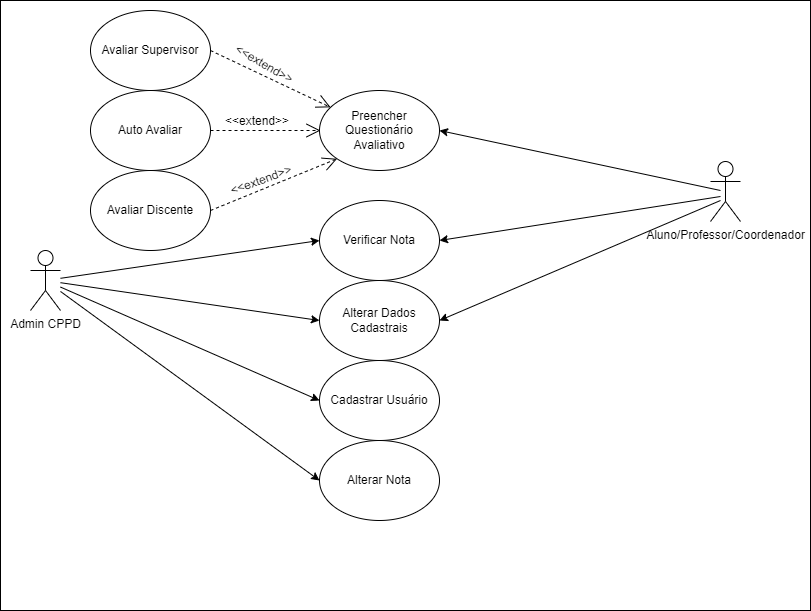
\includegraphics[width=0.99\textwidth]{./img/CasoUso.png}
    \caption{Diagrama de Caso de Uso.}
    \label{fig:CasoUso}
    \end{figure}
  
    Este diagrama possui dois atores que são Admin CPPD e Aluno/Professor/Coordenador e demonstra a perspectiva que os usuários possuíram no SAD, os oito casos de usos evidencia as funções, possuindo também os \textit{extend} que é utilizada para incluir um comportamento opcional de um caso de uso extensor para um caso de uso estendido.

    O propósito do documento abaixo é apresentar a relação e descrição sucinta dos casos de uso do sistema. Fornecendo uma descrição clara e consistente do que o sistema deverá fazer, consistindo na explicitação de todas as diferentes funcionalidade do sistema, que permitirá inferir e identificar mais claramente outras necessidades.

    \begin{figure}[h]
    \centering
    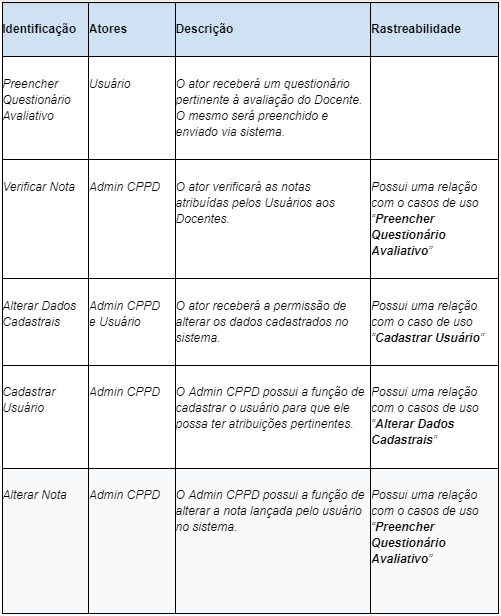
\includegraphics[width=0.85\textwidth]{./img/DescricaoCasoUso.png}
    \caption{Descrição do Casos de Uso.}
    \label{fig:DescricaoCasoUso}
    \end{figure}
  
\section{Recomendações Ágil} 

    Seguindo as boas práticas de desenvolvimento é utilizado a ferramenta Trello para o desenvolvimento de um quadro Kanban para uma gestão ágil do desenvolvimento do Sistema de Avaliação Docente. O quadro Kanban é implementado com o intuito de fornecer e manter informações sobre o desenvolvimento do SAD.

    Nele é incluído as colunas Andamento, Concluído, \textit{Backlog} que se refere o que precisa ser elaborado e o Painel de Controle que auxilia no controle das tarefas. Os recursos da ferramenta são bastante utilizados, podendo definir prazos, critério de prioridade até alertas via e-mail referente a prazos de entregas pendentes. 
    
    \begin{figure}[h]
    \centering
    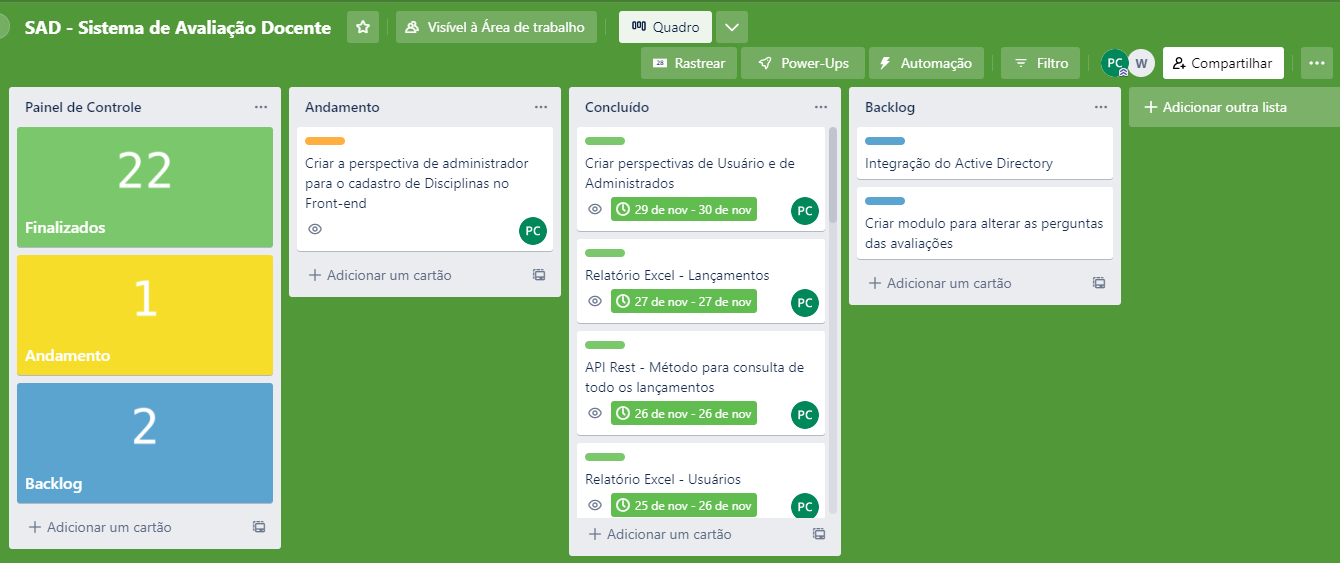
\includegraphics[width=1.0\textwidth]{./img/TrelloSad.png}
    \caption{Quadro Kanban do Sistema de Avaliação Docente,}
    \label{fig:TrelloSad}
    \end{figure}
    
    Com isso é estruturado um cenário que definia os \textit{Sprint Backlog}, o \textit{Time Box} e o \textit{Product Backlog} do Scrum, assim é aplicado as recomendações ágil e as práticas e técnicas que são suportadas, usufruindo as melhores abordagens para um cenário de desenvolvimento.

\section{Estrutura e Arquitetura do Banco de Dados}    

    \begin{figure}[h]
    \centering
    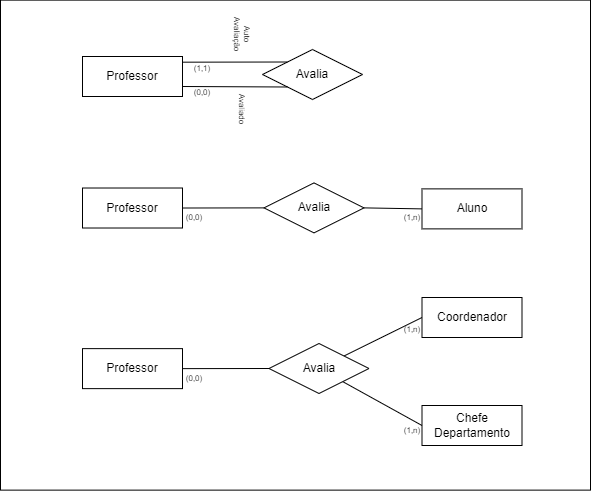
\includegraphics[width=0.60\textwidth]{./img/ModeloEntidadeRelacionamento.png}
    \caption{Diagrama de Entidade Relacionamento.}
    \label{fig:ModeloEntidadeRelacionamento}
    \end{figure}
    
    A fim de estruturar o banco de dados é constituída a estrutura de tabelas conforme demonstrado diagrama de entidade relacional na figura acima. O modelo conceitual demonstra os relacionamentos de avaliações feitas por um docente do Instituto Federal de Goiás e apresenta um diagrama de entidade relacionamento, em que são identificados os relacionamentos entre as entidades e suas cardinalidades. Também são apresentados para cada entidade suas chaves primárias e secundárias bem como seus dados.
    
    \begin{figure}[h]
    \centering
    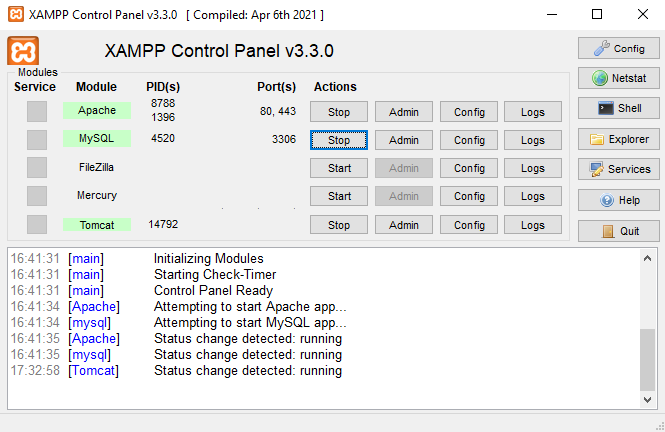
\includegraphics[width=0.75\textwidth]{./img/XAMPP.png}
    \caption{Execução XAMPP.}
    \label{fig:XAMPP}
    \end{figure}
    
    A utilização do sistema XAMPP como ferramenta de gerenciamento do \textit{Apache, MySQL e Tomcat}, auxiliou a utilização do \textit{PhpMyAdmin} no servidor \textit{web Windows}. O XAMPP inicia localmente o \textit{PhpMyAdmin} que por sua vez está armazenado o banco de dados sad com suas respectivas tabelas. A imagens acima mostra a sua inicialização com algumas informações importantes em sua interface, como: Quais serviços estão em execução, portas utilizadas, além de um controle de logs e um painel de configuração que auxiliar em sua manutenção.

    \begin{figure}[h]
    \centering
    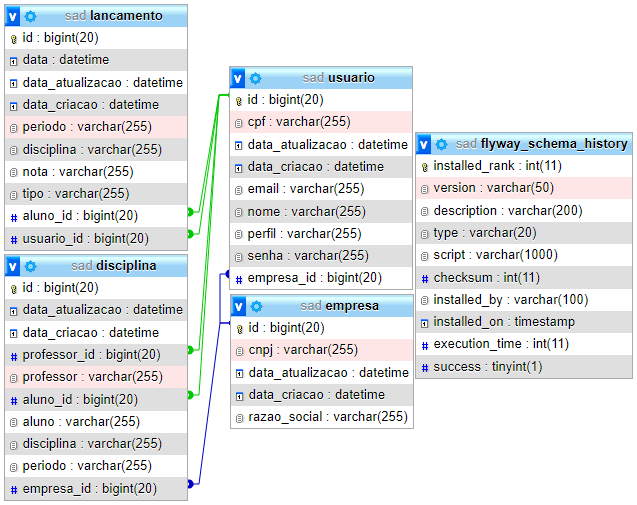
\includegraphics[width=0.77\textwidth]{./img/ModeloFisico.png}
    \caption{Modelo Físico.}
    \label{fig:ModeloFisico}
    \end{figure}
    
    Na imagem acima demonstra como está modelado o banco de dados sad e suas respectivas tabelas, contendo: usuario, empresa, lacamento, disciplina e flyway\_schema\_history. Sendo que os relacionamentos feitos entre as tabelas, são realizados entre as chaves primárias e a chaves estrangeiras, construindo um banco de dados mais seguro evitando possíveis registros duplicados, pois os registros serão únicos dentro da tabela determinada pelas chaves.
        
    Já a tabela flyway\_schema\_history é responsável pelo controle e possui funções essenciais com o \textit{backend} do sistema SAD. A flyway\_schema\_history é uma tabela de histórico de esquema do banco de dados, ela é populada a partir que a \textit{API RESTfu}l quando o \textit{flyway} começa a escanear o sistema e localiza os arquivos SQL no diretório destinado, efetuando as migrações para SGBD, que gerará um histórico do esquema com as versões migradas, de acordo com a implementação.
        
    \begin{figure}[h]
    \centering
    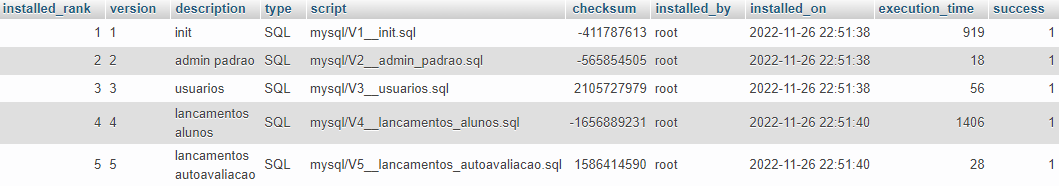
\includegraphics[width=1.0\textwidth]{./img/FlywaySchema.png}
    \caption{Tabela de Histórico de Esquema.}
    \label{fig:ModeloFisico}
    \end{figure}
    
    Os registros da tabela flyway\_schema\_history guardam o histórico de arquivos imputados no banco de dados do sad. Armazenando o nome do arquivo, tipo, versão, data e tempo da execução e se foi executado com sucesso, conforme evidenciado na imagem acima. 

    
\section{Desenvolvimento da API RESTful}

    Para que se possa entender o que foi desenvolvido na \textit{API RESTful} do SAD, o modelo abaixo demonstrará a arquitetura implantada. Primeiro mostra o armazenamento no banco de dados utilizando \textit{PhpMyAdmin} e o \textit{Flyway} para o gerenciamento do banco de dados, que será também responsável pelas migrações e controle do MySQL. Após o \textit{JPA Repository}, que faz parte da \textit{API Spring Data} e possui a função de fornecer o acesso ao banco e a algumas entidades JAVA padrão.
  
    \begin{figure}[h]
    \centering
    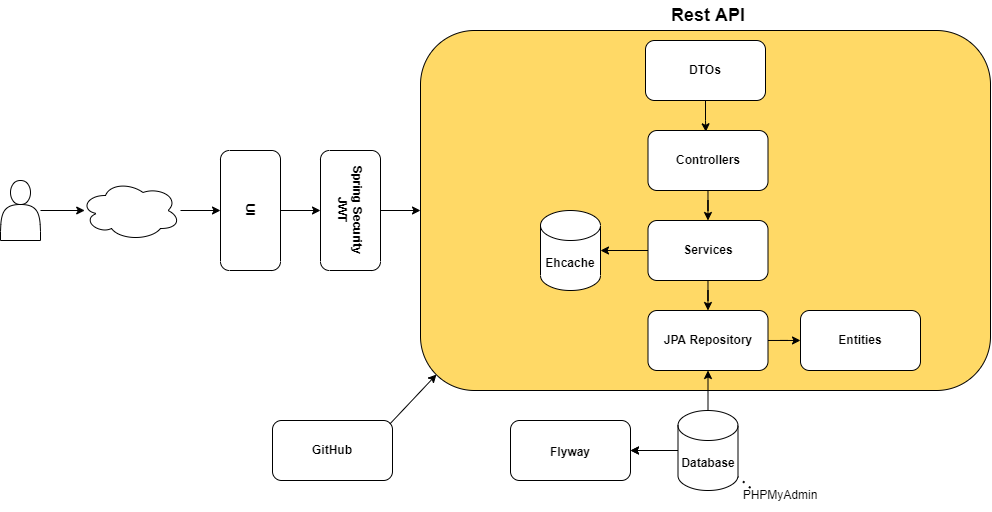
\includegraphics[width=0.90\textwidth]{./img/ArquiteturaRESTAPI .png}
    \caption{Arquitetura da API RESTful.}
    \label{fig:Arquitetura}
    \end{figure}
    
    Para comunicação entre o \textit{JPA Repository} e o banco de dados, existe uma camada de serviços que possui como função as regras de negócio da aplicação, em \textit{Services} também possui uma unidade de \textit{cache}, para fazer o cache de serviços evitando ou melhorando a performance, utilizando da distribuição \textit{JAVA Ehcach}. Para as chamadas ao \textit{Services}, os \textit{Controllers} serão responsáveis e farão a interface com Services e também fará o uso dos \textit{Data Transfer Object} (DTOs) para a comunicação com o cliente. Todos os dados recebidos e enviados serão convertidos em DTOs.
    
    A comunicação feita pelo usuário através da interface gráfica que é chamada de UI (Interface de Usuário), acessada pela Internet, fará o uso dos Controllers. Porém entre essa comunicação existe uma API de Segurança chamada \textit{Spring Security} com a autenticação via \textit{tokens} em JWT. E para armazenamento do código-fonte está sendo utilizado o GitHub,  que permite a hospedagem prática na nuvem, podendo compartilhar o código-fonte.

   Uma boa documentação de uma \textit{API REST} é crucial para desenvolvedores, testadores, mantenedores entenderem claramente o comportamento fornecido por ela. Sendo capaz de apoiar o time nas etapas de desenvolvimento, compreensão e manutenção de código. 
    
    A ferramenta que foi utilizada é o Swagger UI, uma interface funcional também foi disponibilizada para a API, abaixo a interface do Swagger UI da \textit{API RESTful} do Sistema de Avaliação de Desempenho Docente, desenvolvida para documentar a solução, destrinchando cada método utilizado.

    
    \begin{figure}[h]
    \centering
    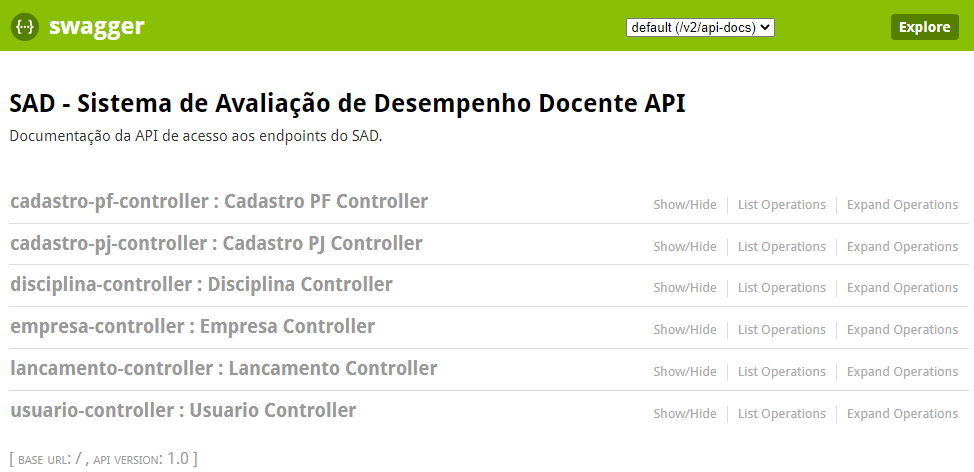
\includegraphics[width=0.81\textwidth]{./img/Swagger.png}
    \caption{Documentação Swagger.}
    \label{fig:Swagger}
    \end{figure}

    \begin{figure}[h]
    \centering
    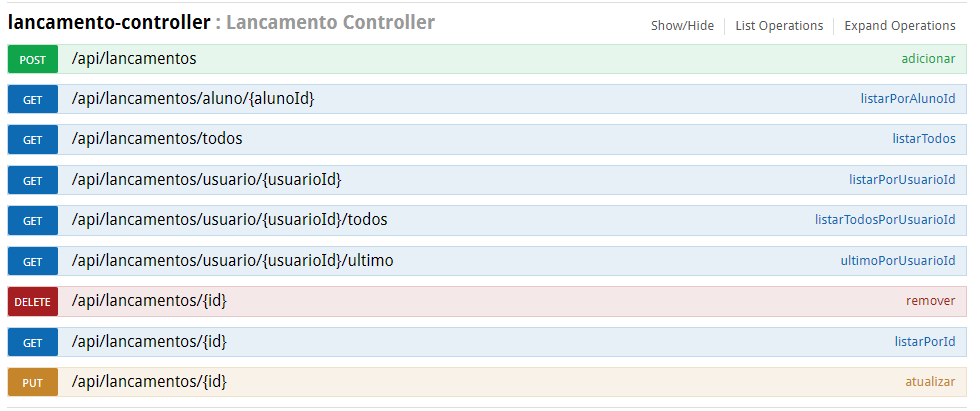
\includegraphics[width=0.81\textwidth]{./img/SwaggerLancamento.png}
    \caption{Documentação Swagger - Lançamento Controller.}
    \label{fig:SwaggerLancamento}
    \end{figure}
    
    A listagem dos métodos de \textit{Lancamento Controller} acima, mostra como está parametrizado cada método para o lançamento das notas do SAD, evidenciando todas a listagens para as consultas das notas, desde de todas as notas lançadas ou as notas de um usuário ou até mesmo a última nota de um usuário, passando também pelos métodos de inclusão, alteração e exclusão. Uma forma de manter a \textit{API RESTful} do SAD bem estruturada e compreensível para os futuros responsáveis pelo \textit{software}.
    
    Para efetuar os testes da API no momento do desenvolvimento foi utilizada a ferramenta Postman, a ferramenta possui como função a chamada do método para efetivação da requisição desejada. Cada método possui seu tipo e parâmetros  de acordo com a requisição, será evidenciado alguns tipos que foram criados para a \textit{API RESTful} do SAD.

    \begin{figure}[h]
    \centering
    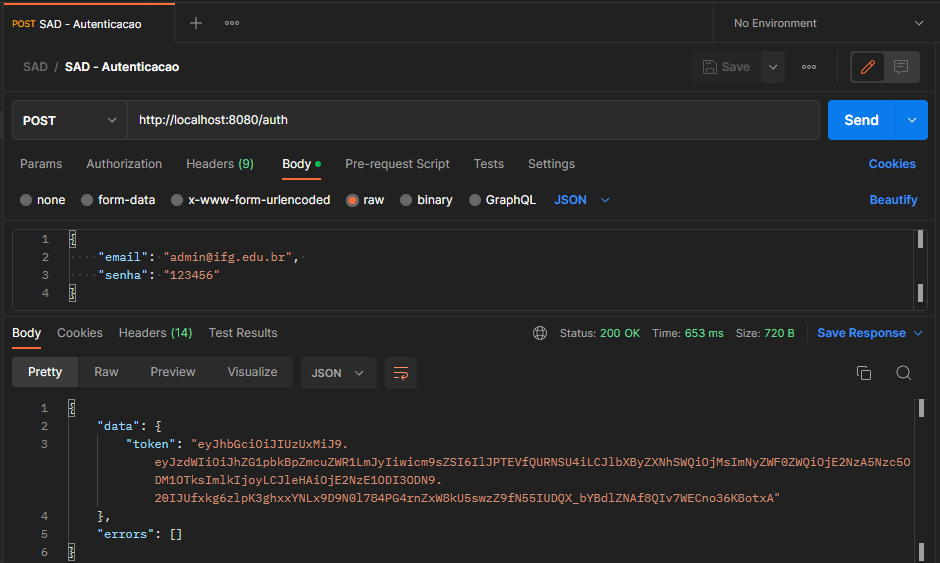
\includegraphics[width=0.72\textwidth]{./img/ApiAutenticacao.png}
    \caption{Método de Autenticação.}
    \label{fig:ApiAutenticacao}
    \end{figure}

    Primeiro para que consiga acessar os métodos é necessário a autenticação passando como parâmetro o usuário e senha disponível no banco de dados. Após a chamada do método é retornado o \textit{token} de autenticação que poderá ser utilizado nas demais requisições. Acima a imagem evidencia como é feita a chamada do endereço, com os parâmetros no JSON para a consulta.
    
    \begin{figure}[h]
    \centering
    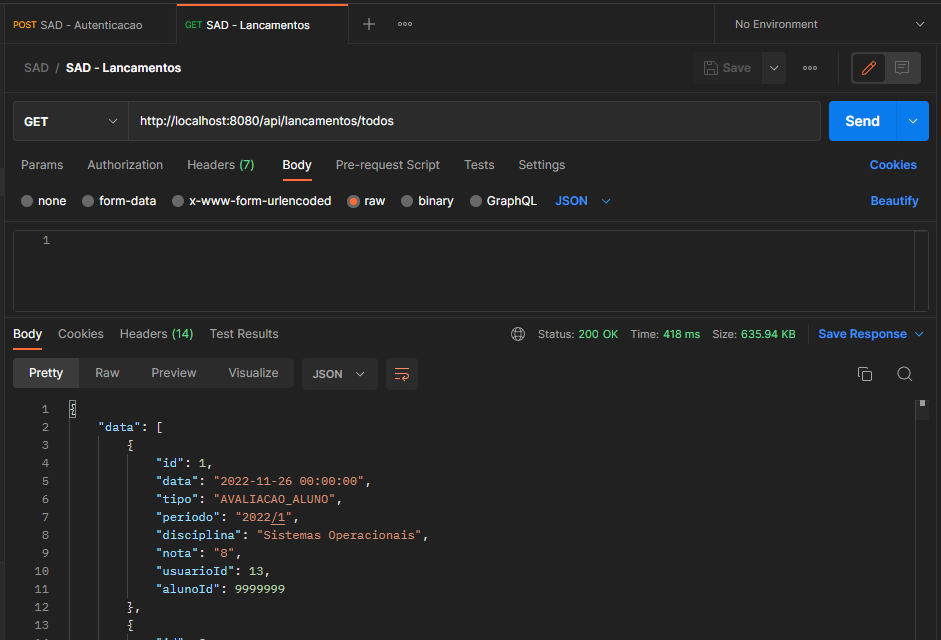
\includegraphics[width=0.72\textwidth]{./img/ApiLancamento.png}
    \caption{Método de Consultar Lançamentos.}
    \label{fig:ApiLancamento}
    \end{figure}

    Após para que consiga efetuar a requisição nos demais métodos é necessário informar o \textit{token} no cabeçalho informando a chave e o valor conforme parametrizado na API, logo efetuando a chamada do endereço com os demais parâmetros necessários conseguirá  efetuar a requisição. O exemplo a seguir evidencia a chamada do método de consulta das notas lançadas do SAD armazenadas no banco de dados, para as demais requisições basta seguir conforme a documentação parametrizada no Swagger.
    
\section{Interface e Funcionalidades do Sistema de Avaliação Docente (SAD)}
    
    No desenvolvimento das interfaces web do Sistema para Avaliação de Desempenho Docente, a aplicação possui como objetivo facilitar a experiência do usuário e estimular sua interação com a solução. Abaixo será demonstrado como o desenvolvimento das interfaces ficaram estruturadas.
    
        \begin{figure}[h]
        \centering
        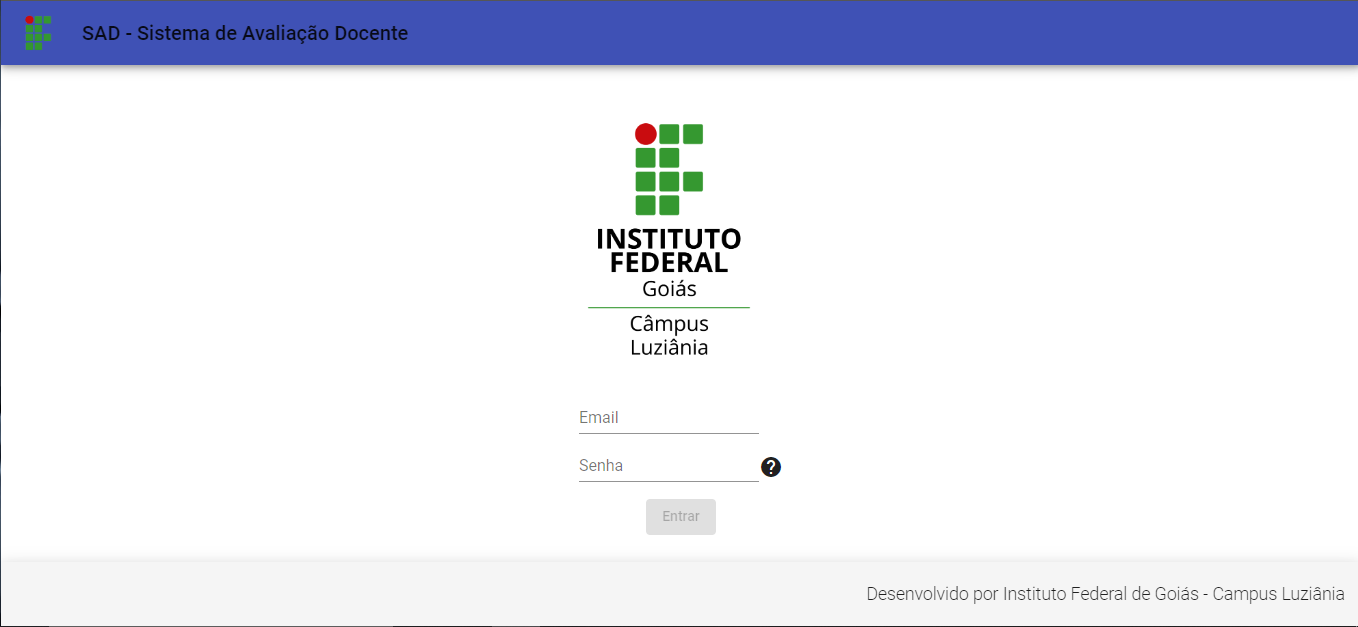
\includegraphics[width=0.94\textwidth]{./img/Login.png}
        \caption{Interface - Tela de Login.}
        \label{fig:Login}
        \end{figure}

    O SAD possui a tela da Figura 27 como tela de Login, a interface permite que o usuário acesse a plataforma, inserindo o e-mail e senha adquiridos através de um cadastro de usuário. Mantém também uma validação se é um e-mail válido e se existe no mínimo 6 caracteres no campo senha, somente a partir dessas validações habilita o botão entrar.
    
        \begin{figure}[h]
        \centering
        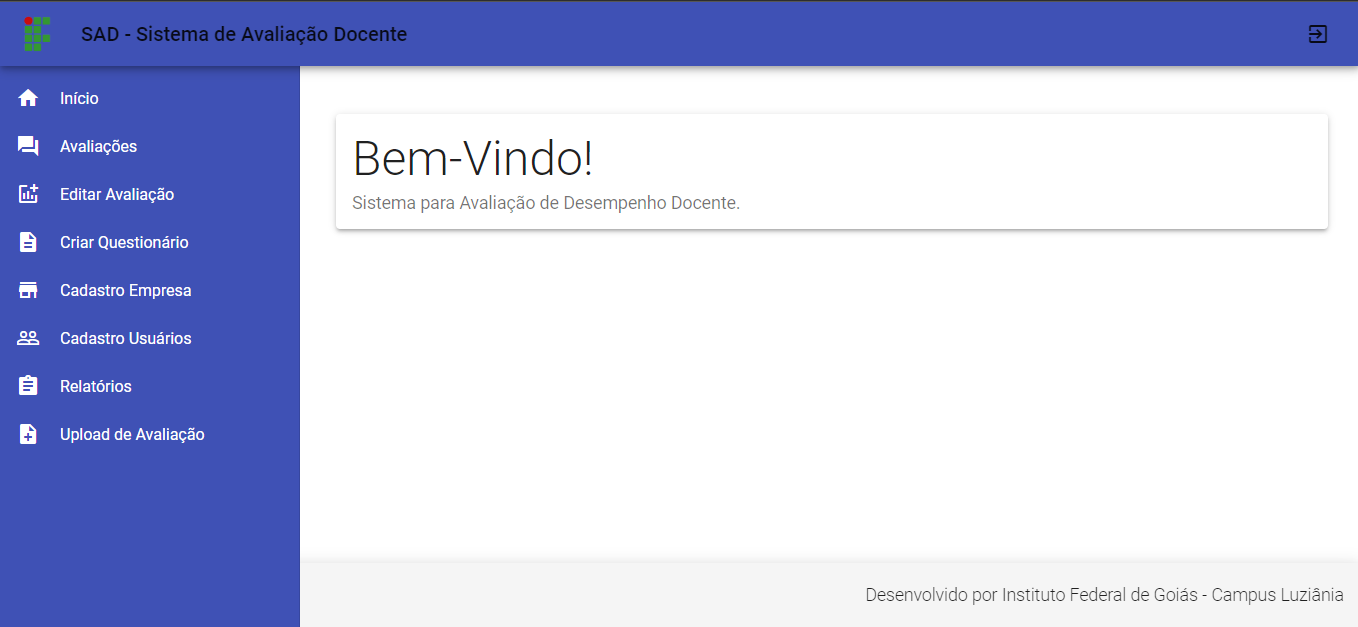
\includegraphics[width=0.94\textwidth]{./img/Home.png}
        \caption{Interface - Tela Inicial - Adminitrador.}
        \label{fig:Inicial}
        \end{figure}

        \begin{figure}[h]
        \centering
        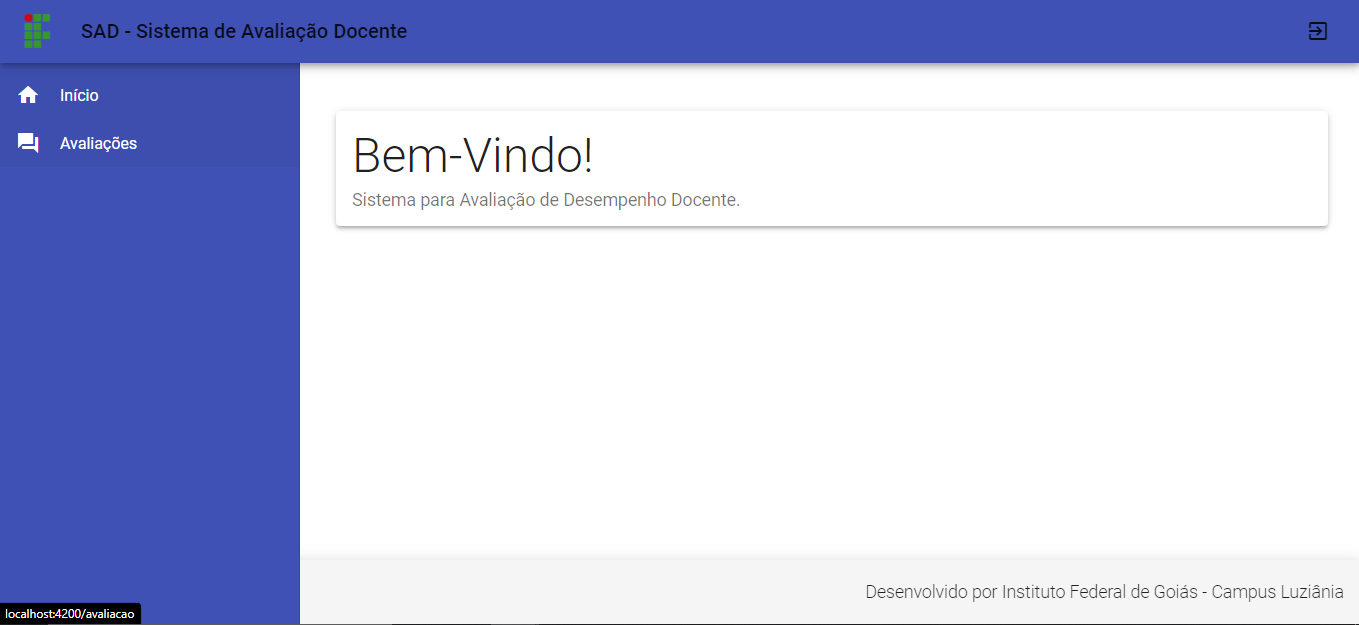
\includegraphics[width=1.0\textwidth]{./img/HomeDiscente.png}
        \caption{Interface - Tela Inicial - Discente.}
        \label{fig:HomeDiscente}
        \end{figure}
        
    A tela inicial, possui como função recepcionar o usuário que está acessando o SAD, seja ele docente, discente, coordenador ou administrador e desejar uma mensagem que seja bem-vindo. Nessa interface já consegue-se observar que os menus estarão disponíveis de acordo com o nível de acesso de cada usuário.     
     
    Também possui uma tela de avaliação para cada tipo de usuário, sendo liberado de acordo com o questionário que será respondido. A tela de avaliação possui a principal função do sistema, onde são feitas as avaliações, na primeira tela carrega os dados do avaliador com o nome e campus, juntamente com a data e hora atual e as disciplinas que estão pendentes para avaliar. 
 
        \begin{figure}[h]
        \centering
        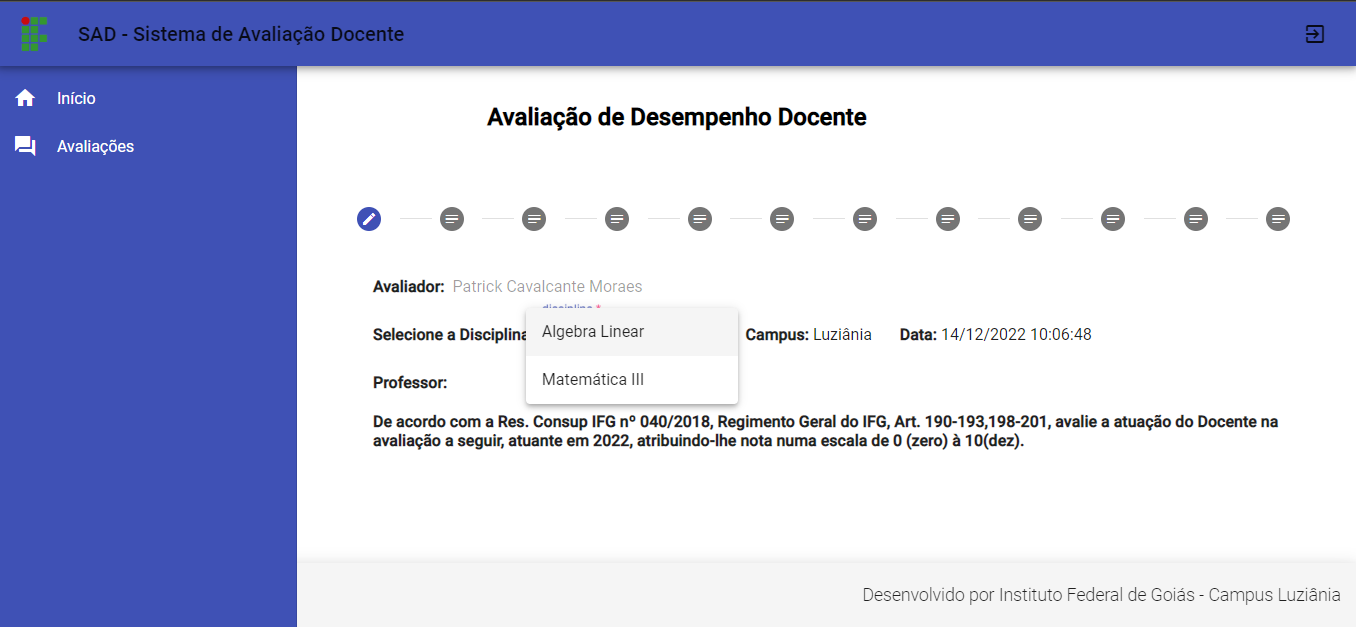
\includegraphics[width=1.0\textwidth]{./img/AvaliaçõesDocente.png}
        \caption{Interface - Tela de avaliações com a seleção da disciplina.}
        \label{fig:Selececao}
        \end{figure}
        
    Juntamente é carregado o regimento pertencente às avaliações docentes do Instituto Federal de Goiás, após o usuário possuirá a opção de selecionar  a disciplina que carregará o docente que será avaliado, conforme as imagens abaixo. 
    
    Essa interface busca ser relativamente fácil de aprender e utilizar, o usuário tem várias abas para a interação com o sistema, é possível alternar de uma aba para outra. O projeto centrado no usuário é uma abordagem de projeto de interface onde a análise das atividades do usuário é primordial para o sucesso do projeto como um todo. A interação dos usuários e a apresentação de informação foram integradas em uma formulação coerente de interface.

    
        \begin{figure}[h]
        \centering
        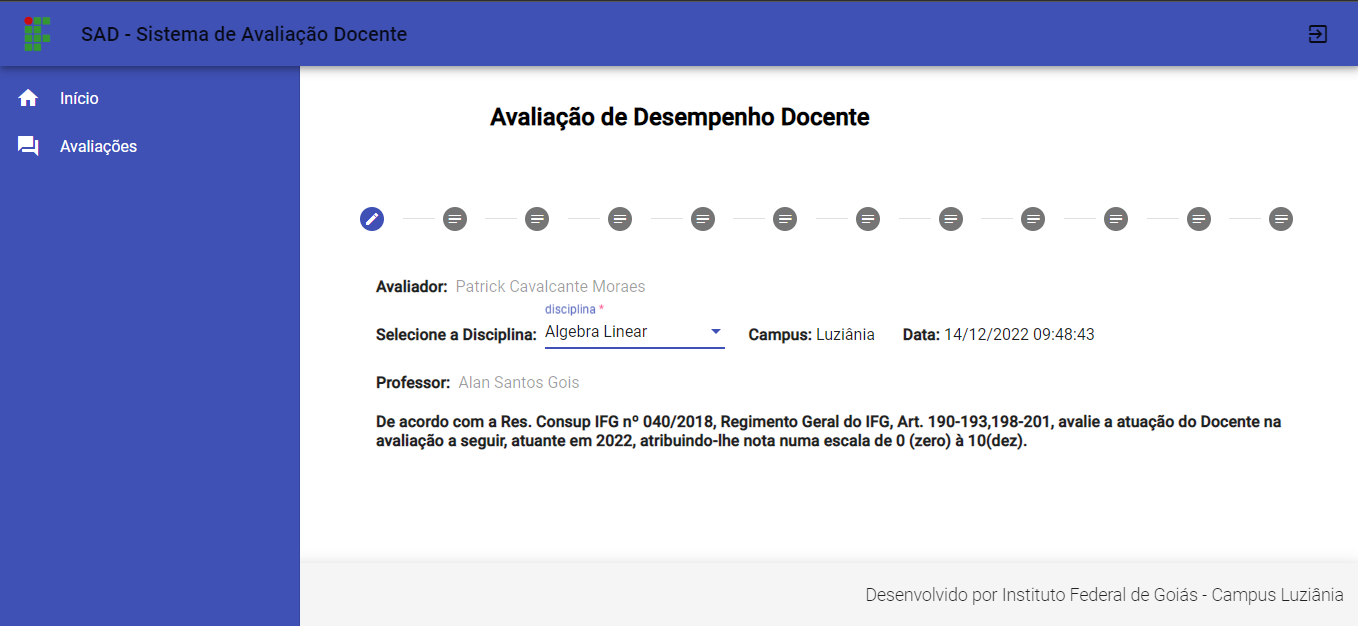
\includegraphics[width=1.0\textwidth]{./img/Avaliações.png}
        \caption{Interface - Tela inicial das avaliações.}
        \label{fig:InicialAv}
        \end{figure}
        
    Após todo o preenchimento do questionário de forma linear, atribuindo uma nota de 0 à 10 em cada resposta, conforme demonstrado na imagem abaixo. Será liberado na última aba, uma confirmação se o usuário deseja enviar o questionário, juntamente com um botão de enviar que possui a função de fazer um requisição na \textit{API RESTful}.  

        \begin{figure}[h]
        \centering
        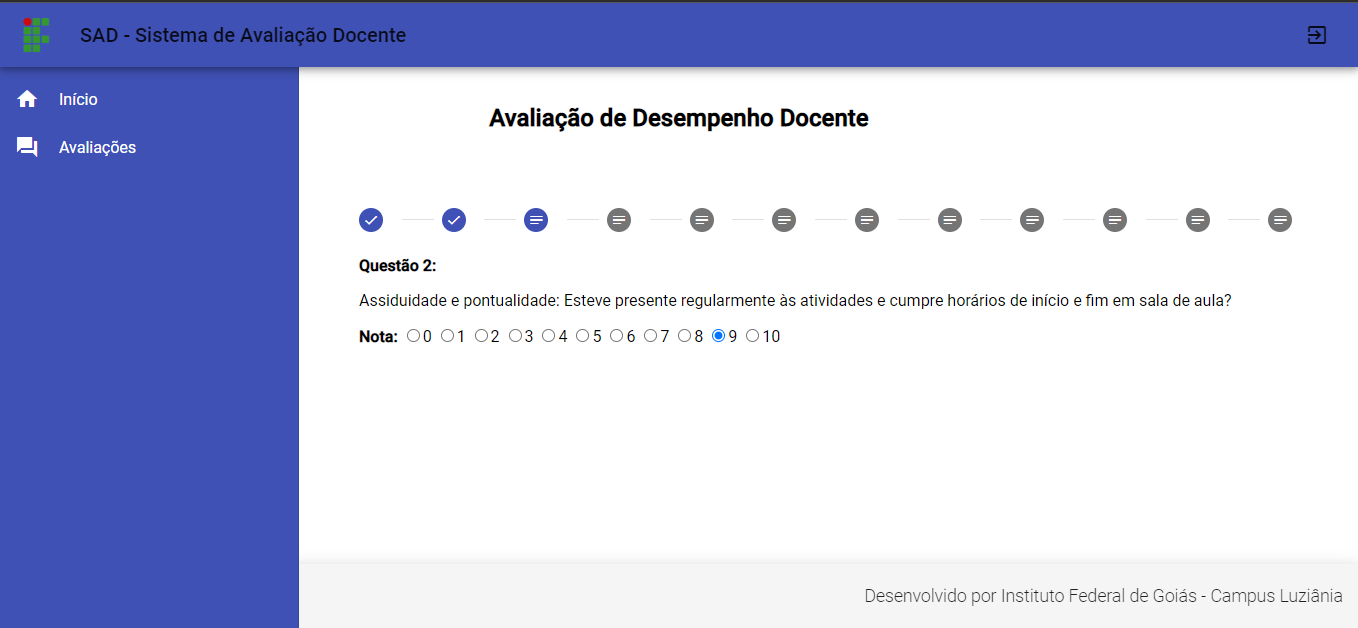
\includegraphics[width=1.0\textwidth]{./img/AvaliaçõesNota.png}
        \caption{Interface - Tela de avaliações com a opção para preencher a nota.}
        \label{fig:Nota}
        \end{figure}

    Caso não seja preenchido algum campo mostrará um alerta informando o campo necessário para o preenchimento, somente após preenchimento de todos os campos conseguirá enviar o formulário. Essa validação é importante, evitando que ocorra registro com informações pendentes no momento do envio da avaliação.
   
    Efetuado o envio da avaliação de desempenho do docente selecionado, o sistema efetuará uma validação e disponibilizará na lista de docentes do usuário, somente os docentes que estão pendente a ser avaliados, uma validação que também é importante, pois evita a duplicidade de registros armazenados no banco de dados.
 
        \begin{figure}[h]
        \centering
        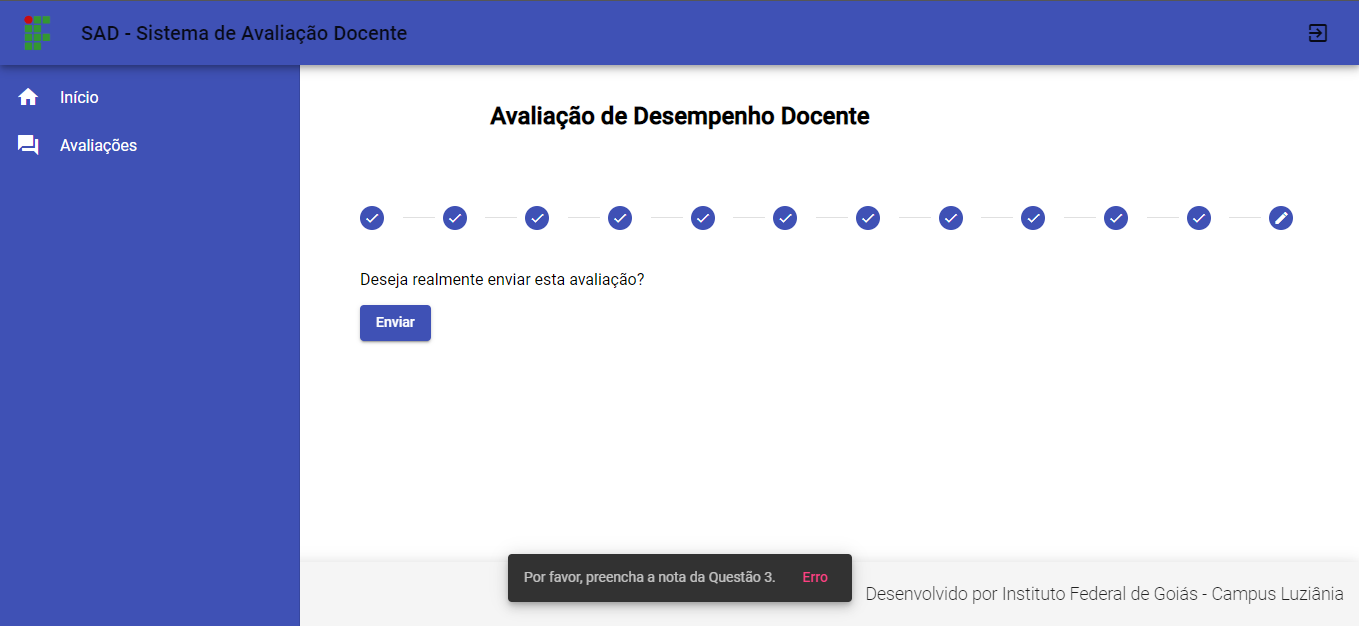
\includegraphics[width=1.0\textwidth]{./img/AvaliaçõesAlerta.png}
        \caption{Interface - Tela de avaliações com o alerta de pendência de campo preenchido.}
        \label{fig:Alerta}
        \end{figure}

    Juntamente com a tela de listar os questionários, que são listados a partir de um filtro que necessita atribuir o docente as quais deseja verificar as notas. A tela oferece algumas opções de ação como a de edição e exclusão da nota lançada para o usuário que possui permissão de administrador. Essa interface também permite a ordenação e paginação dos lançamentos de acordo com a necessidade do usuário.

        \begin{figure}[h]
        \centering
        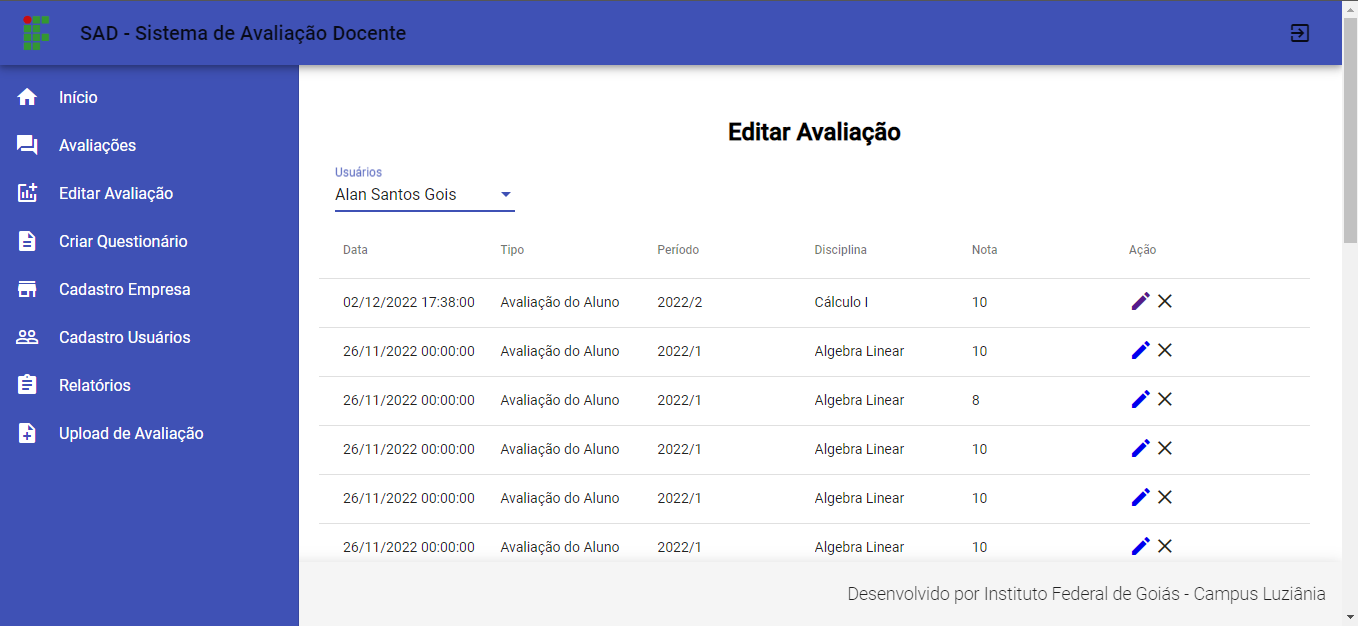
\includegraphics[width=1.0\textwidth]{./img/EditarNotas.png}
        \caption{Interface - Tela de listar notas.}
        \label{fig:EditarNota}
        \end{figure}
        
    A paginação permite que as informações sejam quebradas entre páginas, com o intuito de evitar uma enorme quantidade de dados e ter uma página enorme, cheia de registros. Já a ordenação, consegue organizar os resultados de acordo com uma ou mais colunas da tabela, podendo definir a ordem dos resultados como crescente ou decrescente.

        \begin{figure}[h]
        \centering
        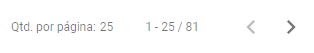
\includegraphics[width=0.45\textwidth]{./img/Paginacao.png}
        \caption{Interface - Paginação.}
        \label{fig:Paginacao}
        \end{figure}

        \begin{figure}[h]
        \centering
        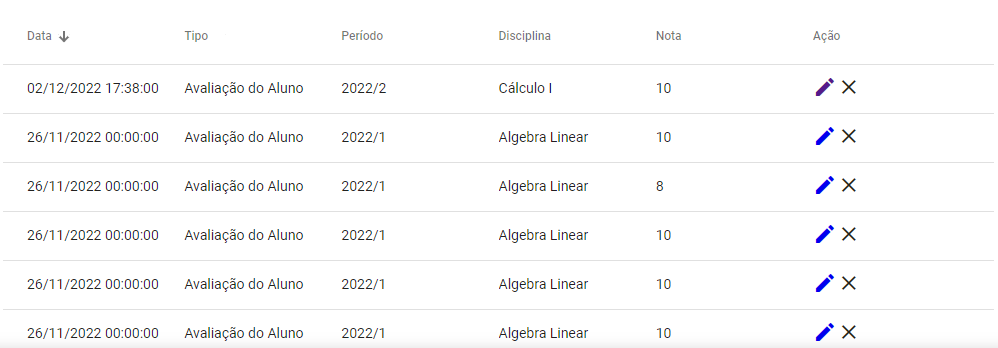
\includegraphics[width=1.0\textwidth]{./img/Ordenacao.png}
        \caption{Interface - Ordenação.}
        \label{fig:Ordenacao}
        \end{figure}

    A ordenação acima demonstra o campo da data sendo ordenado de forma crescente. Caso seja chamada a função de edição, retornará a tela que o administrador conseguirá fazer as alterações necessárias nos campos data, horas, minutos e nota juntamente com as demais informações para consulta.

        \begin{figure}[h]
        \centering
        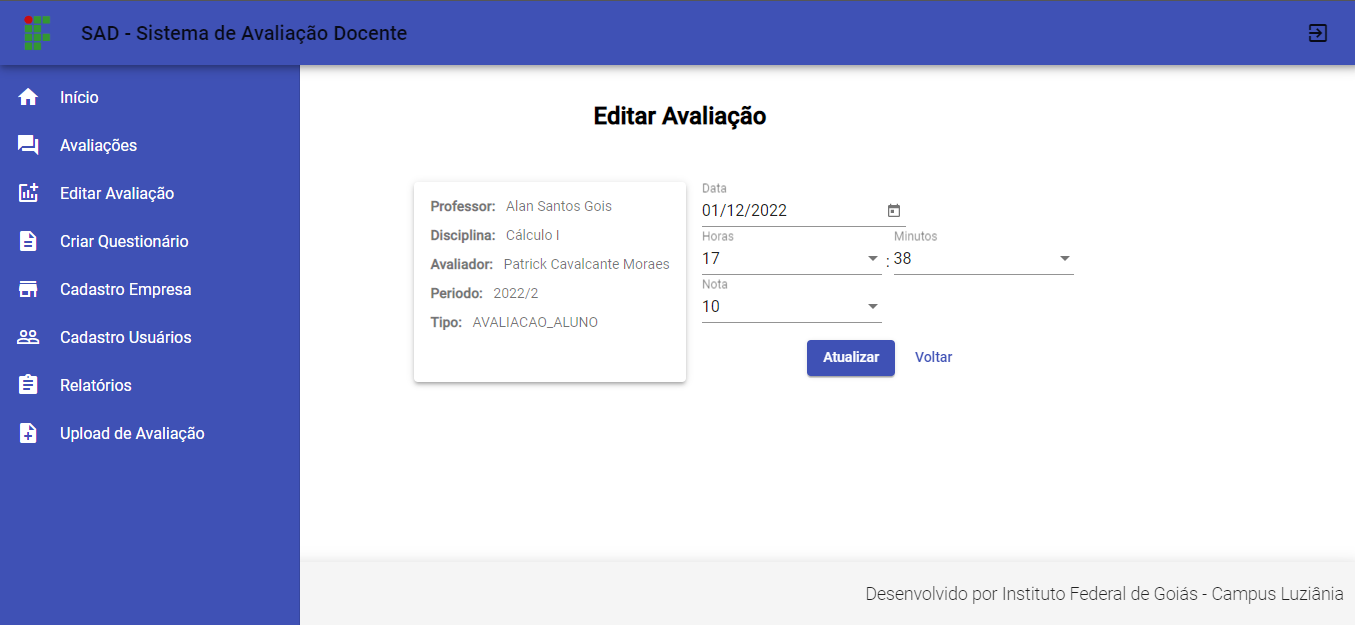
\includegraphics[width=1.0\textwidth]{./img/Editar.png}
        \caption{Interface - Tela de editar notas.}
        \label{fig:Editar}
        \end{figure}
    

    Os cadastros que somente o usuário com privilégio de administrador pode acessar, estão nas interfaces cadastrar empresa e usuários. O cadastrar empresa possui uma classe em JavaScript de validação do CNPJ e CPF, onde são aceitos somente CNPJ e CPF válidos. Os demais campos são o de Razão Social, Nome, E-mail e Senha, com validações de 6 dígitos no campo Senha e validação de e-mail no campo E-mail.
    
    Após a efetuação do cadastro da empresa este CNPJ cadastrado deverá ser vinculado aos usuário de acordo com a empresa que ele atua. Este cenário existente, fará a validação do usuário pertencente a cada instituto e a segregação dos usuários. No cadastro do usuário além dos campos necessário comparados com o do cadastro da empresa que são CNPJ da empresa, CPF, E-mail e Senha válidos. Existe o campo Função que possui como atribuição a diferenciação dos níveis de acesso do usuário, essas funções são denominadas no SAD como Aluno, Professor e Coordenador/Chefe Dep.


        \begin{figure}[h]
        \centering
        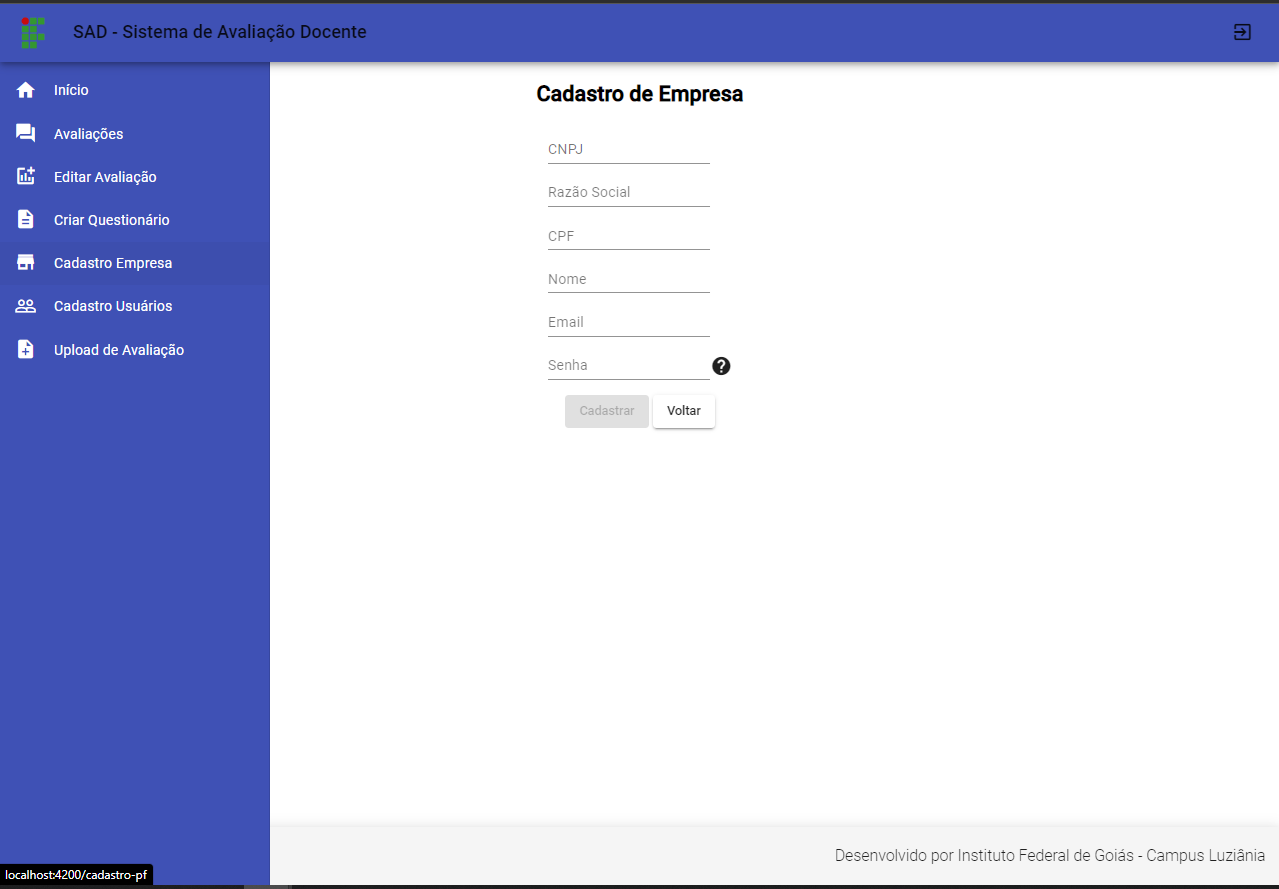
\includegraphics[width=1.0\textwidth]{./img/Empresa.png}
        \caption{Interface - Tela de cadastrar empresas.}
        \label{fig:Empresas}
        \end{figure}
        
        \begin{figure}[h]
        \centering
        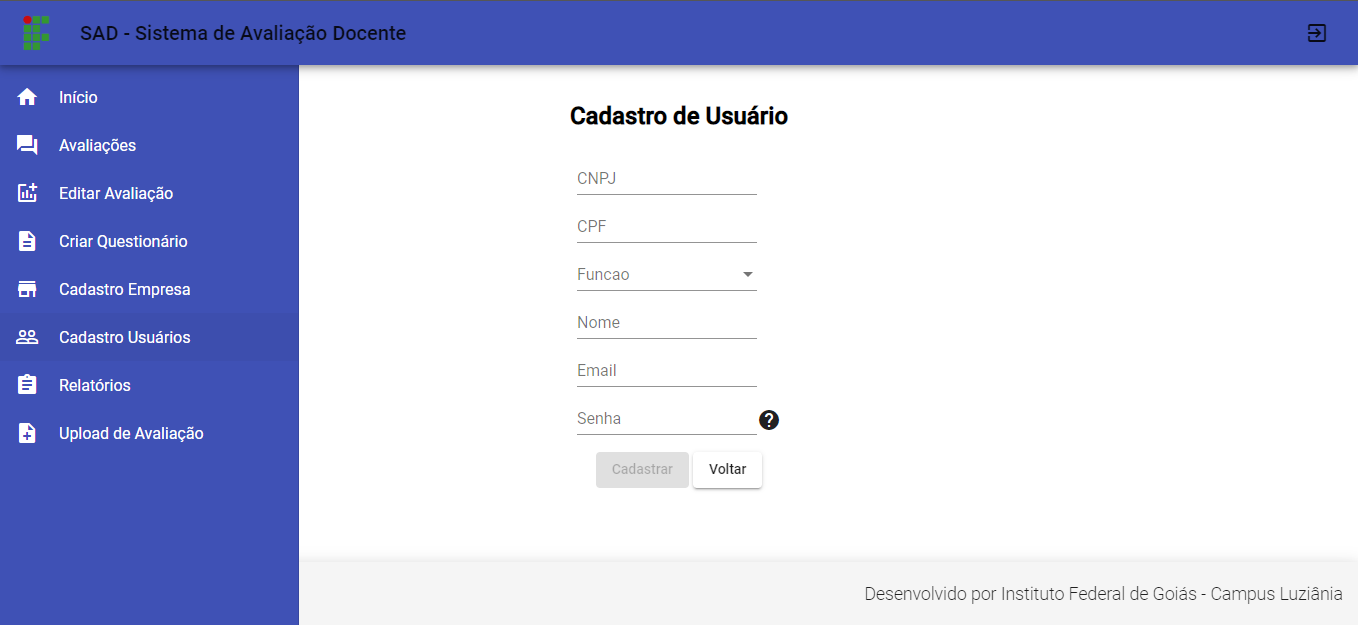
\includegraphics[width=1.0\textwidth]{./img/Usuario.png}
        \caption{Interface - Tela de cadastrar usuários}
        \label{fig:Usuario}
        \end{figure}

        A fim de apresentar os resultados de acordo com a necessidade e uma forma fácil para extração das informações, foi criado o módulo que efetua a geração dos relatórios do sistemas. Disponibilizando os relatórios do cadastro de usuário, das disciplinas e das notas lançadas para os docentes, possuindo também a função para extração do relatório em CSV.

        \begin{figure}[h]
        \centering
        \includegraphics[width=1.0\textwidth]{./img/relatorio.png}
        \caption{Interface - Relatório das notas lançadas para os docentes.}
        \label{fig:relatorio}
        \end{figure}

        Sendo assim, os relatórios gerenciais tomaram um papel muito importante e são a principal forma de analisar as informações da Avaliação de Desempenho Docente, possibilitando uma tomada de decisão mais ágil, reduzindo riscos e expondo oportunidades.

    
\section{Testes}

    Baseado nos requisitos levantados juntamente com a Comissão Permanente de Pessoal Docente, foi desenvolvido o Sistema para Avaliação de Desempenho Docente, e para realização dos testes de desempenho e usabilidade do sistema, foram desenvolvidas algumas abordagens para concretização do projeto.
        
    Foi efetuado também na primeira etapa uma reunião para efetivação dos testes de aceitação juntamente com os integrantes da CPPD, com um protótipo já elaborado foram efetuadas abordagens de aceitação, apresentando o protótipo e verificando as necessidades e possíveis melhorias. As necessidades levantadas trouxe uma melhor visão da regra de negócio da instituição, e uma perspectiva dos usuários se o projeto conseguiria atender as necessidade da comissão.  

    Após a concretização dos pontos de função levantados anteriormente, foi apresentado o protótipo final, demonstrando todas as funcionalidades desenvolvidas para o sistema SAD. Essa abordagem foi estabelecida para que consiga efetivar o que foi proposto e disponibilizar o sistema para a implantação no Instituto Federal de Goiás. 

    Com a carga parcial dos dados feita pela \textit{API RESTful}, os membros da CPPD conseguiram visualizar o que foi proposto e desenvolvido, visando trazer um cenário para o ponto de vista que o usuário utilizará, corrigindo eventuais problemas que poderiam ocorrer após á implementado na instituição e com início da utilização do SAD. 
    
    Durante o processo de desenvolvimento foi utilizado o conceito de TDD, que após a criação de cada classe foi implementado um classe teste. Utilizando os recursos do @SpringBootTest com o mecanismo do JUnit para os testes unitários. Para os testes de interação foi implementado armazenamento de persistência H2 na memória que faz a consulta somente dos registros armazenados na memória criados para o teste da classe. 

        \begin{figure}[h]
        \centering
        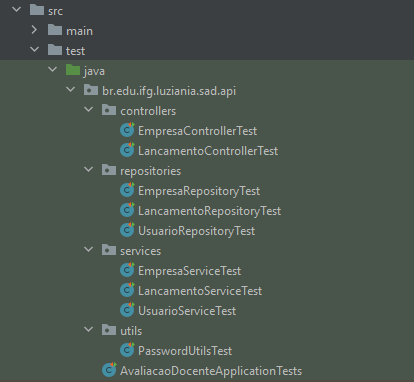
\includegraphics[width=0.38\textwidth]{./img/ClasseTeste.png}
        \caption{Estruturação das Classes de Teste.}
        \label{fig:ClasseTeste}
        \end{figure}

    Na Figura 41 é demonstrado a estrutura das classes teste para \textit{API RESTful} do SAD, as classes foram implementadas e após a execução retorna no terminal o resultado da obtido. Quando os testes forem executados em modo gráfico, os métodos testados podem apresentar os seguintes resultados: verde para sucesso, roxo para exceção  e vermelho para falha.

        \begin{figure}[h]
        \centering
        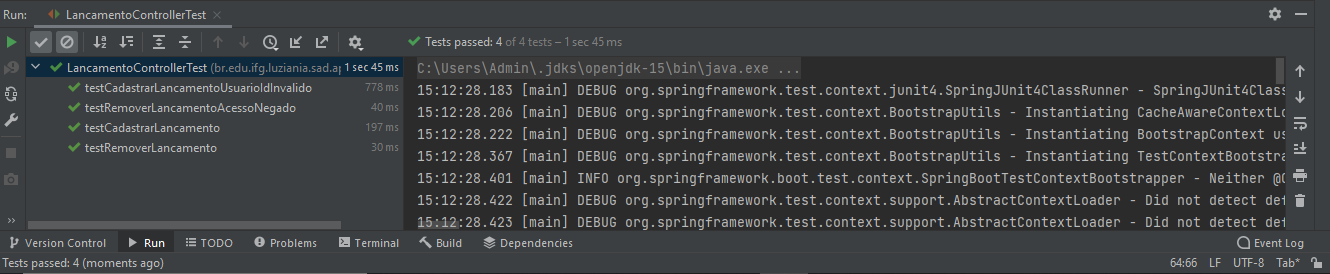
\includegraphics[width=1.0\textwidth]{./img/ClasseTesteTerminal.png}
        \caption{Execução da Classe de Teste LancamentoControllerTest.}
        \label{fig:ClasseTesteTerminal}
        \end{figure}

     Para os testes de desempenho da \textit{API Restful}, foi simulado múltiplos acessos em paralelo, e obteve algumas métricas sobre a execução. Com Apache AB que é um executável que vem junto com o servidor Apache HTTP, e é ideal para testes de performance, e disponibiliza via linha de comando realizar requisições HTTP, permitindo configurar a quantidade de requisições, quantidade de requisições em paralelo, espaço de tempo para realizar as requisições, entre outros. Sendo que no final, ele exibe um relatório com o plano de execução, demonstrando dados e métricas do que foi executado. 

    O Apache AB está localizado dentro do diretório bin da instalação do Apache, e é acessado via linha de comando, com a utilização do terminal do XAMPP. Navegando até o diretório bin dentro da instalação do Apache HTTP Server, foi executado o comando da Figura 43, o comando executará dez mil requisições a URL informada, sendo que com uma concorrência de mil ao mesmo tempo,  ao término da execução será exibido o relatório.
    
        \begin{figure}[h]
        \centering
        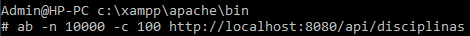
\includegraphics[width=0.60\textwidth]{./img/ComadoRequisicoes.png}
        \caption{Execução do comando para dez mil requisições.}
        \label{fig:ComadoRequisicoes}
        \end{figure}
        
    No relatório de desempenho da Figura 44 é a evidencia a execução das requisições, que são divididas entre mil até completar as dez mil requisições. São mostrado alguns dados, como: nome do host do servidor, porta do servidor, caminho do documento, comprimento do documento, nível de simultaneidade, tempo gasto para testes, pedidos completos, solicitações com falha, total transferido, HTML transferido, solicitações por segundo, tempo por solicitação e taxa de transferência entre outros.

        \begin{figure}[h]
        \centering
        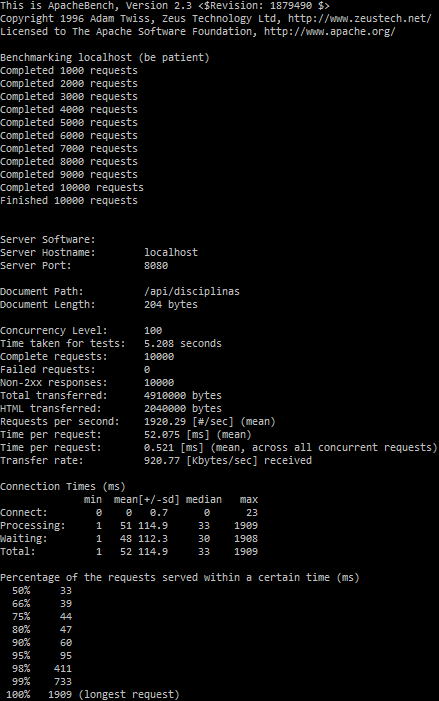
\includegraphics[width=0.65\textwidth]{./img/RelatorioDesempenho.png}
        \caption{Relatório de Desempenho.}
        \label{fig:ComadoRequisicoes}
        \end{figure}
        
    A partir do relatório de desempenho da \textit{API Restful}, pode-se obter que o tempo percorrido de 5.208 segundos para a execução do teste de dez mil requisições que foi adequado para a aplicação, garantindo assim sua qualidade. Assim pode-se prever que a aplicação conseguirá executar dez mil requisições em um tempo hábil sem nenhum tipo de stress ou falha e que os demais dados do relatório estão coerentes para um sistema.
        
    
    
\chapter{CONCLUSÃO}

    A avaliação de desempenho docente demonstra que o Instituto Federal de Goiás está atento com a garantia de desempenho e progressão de seus docentes. Esse trabalho apresentou o Sistema de Avaliação de Desempenho Docente (SAD) para atender com mais qualidade esse processo de avaliação, evidenciando também que o modelo aplicado atualmente já não agregaria resultados satisfatórios diante o cenário atual.

    A solução proposta pode ser implantada para resolver a necessidade de um sistema que contemple as três avaliações do docente, e que consiga integrar essas informações em dados concretos e de fácil manuseio para a Comissão Permanente de Pessoal Docente unificando todo o processo em uma única aplicação.

    A evolução da tecnologia permitiu que os sistemas avançassem cada vez mais no que se refere à solução de problemas e se tornaram mais acessíveis às instituições. O objetivo deste projeto é justamente aproveitar os benefícios da tecnologia para a criação do SAD que poderá fornecer apoio às decisões tornando-as mais eficientes e eficazes, onde o administrador conseguiria coletar e controlar todas as informações e conseguirá utilizá-las da maneira mais adequada. 

    Assim, o que se define como um processo bem sucedido é aquele que cria mudanças claras e duráveis de comportamento e/ou desenvolvimento de habilidades, de modo a promover um incremento na efetividade da organização. Pode-se então concluir que o SAD para avaliação de desempenho docente é essencial para a saúde da instituição e para a uma melhor qualidade de seu serviço. 
    
    
\section{Trabalhos futuros}  
    A contemplação do Sistema de Avaliação Docente dado ao desenvolvimento do SAD conforme abordado neste trabalho, daria-se em sua utilização pelo Instituto Federal de Goiás, logo para que se consiga implementar a ferramenta deve-se seguir algumas aprovações como a da CPPD que já foi avaliada e efetivada positivamente, em seguida pode ser feita a avaliação por parte do Diretoria de Tecnologia da Informação(DTI) do IFG para sua implementação. O SAD possui algumas funcionalidades que ainda necessitam ser desenvolvidas, como a integração do \textit{Active Directory}(AD) para o controle de acessos, uma das melhorias que pode ser feita é a criação da integração do SAD com o AD.

    O SAD também é uma ferramenta que foi proposta para ser facilmente adaptada para outros sistemas de avaliações de desempenho. Como trabalhos futuros, podem ser desenvolvidos a partir desse sistema outros sistemas de apoio à decisão que pode ser implantado em diversas instituições públicas ou privadas.
    
% \chapter{Recursos Necessários}

% Os recursos necessários para a criação do Sistema para Avaliação de Desempenho serão:
    
% \begin{itemize}
   %  \item Computador com configuração mínima de, 3.0 GHz de processamento, 4Gb de RAM, 2Gb de espaço livre no HD;
   %  \item Papel Sulfite e cartuchos para impressão do trabalho;
   %  \item Internet para realizar as pesquisas;
   %  \item Sofware IDE de Desenvolvimento Intellij e Visual Studio Code.
   %  \item XAMPP responsável pelo Apache e MySQL.
   %  \item A plataforma OverLeaf para o desenvolvimento do trabalho escrito.
% \end{itemize}



%\chapter{Cronograma}

    %Esta seção apresenta o cronograma deste projeto, como será dividida as atividades dentro do tempo estimulado para a realização deste trabalho. 
    
%\begin{itemize}
   % \item \textbf{Atividade 1:} Fazer o levantamento de requisitos;
    %\item \textbf{Atividade 2:} Modelar os requisitos na forma de diagramas;
   % \item \textbf{Atividade 3:} Elaborar o projeto de software; 
    %\item \textbf{Atividade 4:} Implementar o software;
    %\item \textbf{Atividade 5:} Apresentar o protótipo a CPPD;
   % \item \textbf{Atividade 6:} Validar o protótipo;
    %\item \textbf{Atividade 7:} Efetuar os testes;
    %\item \textbf{Atividade 8:} Escrita do projeto.
%\end{itemize}

    %Abaixo temos a tabela do cronograma a ser seguido:
    


% Tabela 1
%\begin{table}[h]
%    \centering
%% distancia entre a linha e o texto
% {\renewcommand\arraystretch{2}
% \begin{tabular}{ l l l l l l l l l l l l l l l l l l }
%  \cline{1-1}\cline{2-2}\cline{3-3}\cline{4-4}\cline{5-5}\cline{6-6}\cline{7-7}\cline{8-8}\cline{9-9}\cline{10-10}\cline{11-11}\cline{12-12}\cline{13-13}\cline{14-14}\cline{15-15}\cline{16-16}\cline{17%-17}\cline{18-18}  
%    \multicolumn{18}{|p{8.000cm}|}{\textbf{Cronograma} \centering }
%  \\  
%  \cline{1-1}\cline{2-2}\cline{3-3}\cline{4-4}\cline{5-5}\cline{6-6}\cline{7-7}\cline{8-8}\cline{9-9}\cline{10-10}\cline{11-11}\cline{12-12}\cline{13-13}\cline{14-14}\cline{15-15}\cline{16-16}\cline{17-17}\cline{18-18}  
%    \multicolumn{1}{|p{1.590cm}|}{\textbf{Atividade} \centering } &
%    \multicolumn{4}{p{1.000cm}|}{\textbf{Abril} \centering } &
%    \multicolumn{5}{p{1.000cm}|}{\textbf{Maio} \centering } &
%    \multicolumn{4}{p{1.000cm}|}{\textbf{Junho} \centering } &
%    \multicolumn{4}{p{1.000cm}|}{\textbf{Julho} \centering } 
%  \\  
%  \cline{1-1}\cline{2-2}\cline{3-3}\cline{4-4}\cline{5-5}\cline{6-6}\cline{7-7}\cline{8-8}\cline{9-9}\cline{10-10}\cline{11-11}\cline{12-12}\cline{13-13}\cline{14-14}\cline{15-15}\cline{16-16}\cline{17-17}\cline{18-18}  
%   \multicolumn{1}{|p{1.590cm}|}{\textbf{ID} \raggedleft } &
%    \multicolumn{1}{p{0.250cm}|}{1S} &
%    \multicolumn{1}{p{0.250cm}|}{2S} &
%    \multicolumn{1}{p{0.250cm}|}{3S} &
%    \multicolumn{1}{p{0.250cm}|}{4S} &
%    \multicolumn{1}{p{0.200cm}|}{1S} &
%    \multicolumn{1}{p{0.200cm}|}{2S} &
%    \multicolumn{1}{p{0.200cm}|}{3S} &
%    \multicolumn{1}{p{0.200cm}|}{4S} &
%    \multicolumn{1}{p{0.200cm}|}{5S} &
%    \multicolumn{1}{p{0.250cm}|}{1S} &
%    \multicolumn{1}{p{0.250cm}|}{2S} &
%    \multicolumn{1}{p{0.250cm}|}{3S} &
%    \multicolumn{1}{p{0.250cm}|}{4S} &
%    \multicolumn{1}{p{0.250cm}|}{1S} &
%    \multicolumn{1}{p{0.250cm}|}{2S} &
%    \multicolumn{1}{p{0.250cm}|}{3S} &
%    \multicolumn{1}{p{0.250cm}|}{4S}
%  \\  
%  \cline{1-1}\cline{2-2}\cline{3-3}\cline{4-4}\cline{5-5}\cline{6-6}\cline{7-7}\cline{8-8}\cline{9-9}\cline{10-10}\cline{11-11}\cline{12-12}\cline{13-13}\cline{14-14}\cline{15-15}\cline{16-16}\cline{17-17}\cline{18-18}  
%    \multicolumn{1}{|p{1.590cm}|}{\textbf{1} \raggedleft } &
%    \multicolumn{1}{p{0.250cm}|}{\textbf{x} \centering } &
%    \multicolumn{1}{p{0.250cm}|}{\textbf{x} \centering } &
%    \multicolumn{1}{p{0.250cm}|}{ } &
%    \multicolumn{1}{p{0.250cm}|}{ } &
%    \multicolumn{1}{p{0.200cm}|}{ } &
%    \multicolumn{1}{p{0.200cm}|}{ } &
%    \multicolumn{1}{p{0.200cm}|}{ } &
%    \multicolumn{1}{p{0.200cm}|}{ } &
%    \multicolumn{1}{p{0.200cm}|}{ } &
%    \multicolumn{1}{p{0.250cm}|}{ } &
%    \multicolumn{1}{p{0.250cm}|}{ } &
%    \multicolumn{1}{p{0.250cm}|}{ } &
%    \multicolumn{1}{p{0.250cm}|}{ } &
%    \multicolumn{1}{p{0.250cm}|}{ } &
%    \multicolumn{1}{p{0.250cm}|}{ } &
%    \multicolumn{1}{p{0.250cm}|}{ } &
%    \multicolumn{1}{p{0.250cm}|}{ }
%  \\  
%  \cline{1-1}\cline{2-2}\cline{3-3}\cline{4-4}\cline{5-5}\cline{6-6}\cline{7-7}\cline{8-8}\cline{9-9}\cline{10-10}\cline{11-11}\cline{12-12}\cline{13-13}\cline{14-14}\cline{15-15}\cline{16-16}\cline{17-17}\cline{18-18}  
%    \multicolumn{1}{|p{1.590cm}|}{\textbf{2} \raggedleft } &
%    \multicolumn{1}{p{0.250cm}|}{ } &
%    \multicolumn{1}{p{0.250cm}|}{  \centering } &
%    \multicolumn{1}{p{0.250cm}|}{\textbf{x} \centering } &
%    \multicolumn{1}{p{0.250cm}|}{\textbf{x} \centering } &
%    \multicolumn{1}{p{0.200cm}|}{\textbf{x} \centering } &
%    \multicolumn{1}{p{0.200cm}|}{ } &
%    \multicolumn{1}{p{0.200cm}|}{ } &
%    \multicolumn{1}{p{0.200cm}|}{ } &
%    \multicolumn{1}{p{0.200cm}|}{ } &
%    \multicolumn{1}{p{0.250cm}|}{ } &
%    \multicolumn{1}{p{0.250cm}|}{ } &
%    \multicolumn{1}{p{0.250cm}|}{ } &
%    \multicolumn{1}{p{0.250cm}|}{ } &
%    \multicolumn{1}{p{0.250cm}|}{ } &
%    \multicolumn{1}{p{0.250cm}|}{ } &
%    \multicolumn{1}{p{0.250cm}|}{ } &
%    \multicolumn{1}{p{0.250cm}|}{ }
%  \\  
%  \cline{1-1}\cline{2-2}\cline{3-3}\cline{4-4}\cline{5-5}\cline{6-6}\cline{7-7}\cline{8-8}\cline{9-9}\cline{10-10}\cline{11-11}\cline{12-12}\cline{13-13}\cline{14-14}\cline{15-15}\cline{16-16}\cline{17-17}\cline{18-18}  
%    \multicolumn{1}{|p{1.590cm}|}{\textbf{3} \raggedleft } &
%    \multicolumn{1}{p{0.200cm}|}{  \centering } &
%    \multicolumn{1}{p{0.250cm}|}{ } &
%    \multicolumn{1}{p{0.250cm}|}{ } &
%    \multicolumn{1}{p{0.250cm}|}{ } &
%    \multicolumn{1}{p{0.250cm}|}{  \centering } &
%    \multicolumn{1}{p{0.200cm}|}{\textbf{x} \centering } &
%    \multicolumn{1}{p{0.200cm}|}{ } &
%    \multicolumn{1}{p{0.250cm}|}{ } &
%    \multicolumn{1}{p{0.200cm}|}{\textbf{x} \centering } &
%    \multicolumn{1}{p{0.200cm}|}{\textbf{x} \centering } &
%    \multicolumn{1}{p{0.250cm}|}{ } &
%    \multicolumn{1}{p{0.250cm}|}{ } &
%    \multicolumn{1}{p{0.250cm}|}{ } &
%    \multicolumn{1}{p{0.250cm}|}{ } &
%    \multicolumn{1}{p{0.250cm}|}{ } &
%    \multicolumn{1}{p{0.250cm}|}{ } &
%    \multicolumn{1}{p{0.250cm}|}{ }
%  \\  
%  \cline{1-1}\cline{2-2}\cline{3-3}\cline{4-4}\cline{5-5}\cline{6-6}\cline{7-7}\cline{8-8}\cline{9-9}\cline{10-10}\cline{11-11}\cline{12-12}\cline{13-13}\cline{14-14}\cline{15-15}\cline{16-16}\cline{17-17}\cline{18-18}  
%    \multicolumn{1}{|p{1.590cm}|}{\textbf{4} \raggedleft } &
%    \multicolumn{1}{p{0.250cm}|}{ } &
%    \multicolumn{1}{p{0.250cm}|}{ } &
%    \multicolumn{1}{p{0.250cm}|}{ } &
%    \multicolumn{1}{p{0.250cm}|}{ } &
%    \multicolumn{1}{p{0.200cm}|}{ } &
%    \multicolumn{1}{p{0.200cm}|}{  \centering } &
%    \multicolumn{1}{p{0.200cm}|}{ } &
%    \multicolumn{1}{p{0.200cm}|}{ } &
%    \multicolumn{1}{p{0.200cm}|}{\textbf{x} \centering } &
%    \multicolumn{1}{p{0.250cm}|}{\textbf{x} \centering } &
%    \multicolumn{1}{p{0.250cm}|}{ } &
%    \multicolumn{1}{p{0.250cm}|}{ } &
%   \multicolumn{1}{p{0.250cm}|}{ } &
%    \multicolumn{1}{p{0.250cm}|}{ } &
%    \multicolumn{1}{p{0.250cm}|}{ } &
%    \multicolumn{1}{p{0.250cm}|}{ } &
%    \multicolumn{1}{p{0.250cm}|}{ }
%  \\  
%  \cline{1-1}\cline{2-2}\cline{3-3}\cline{4-4}\cline{5-5}\cline{6-6}\cline{7-7}\cline{8-8}\cline{9-9}\cline{10-10}\cline{11-11}\cline{12-12}\cline{13-13}\cline{14-14}\cline{15-15}\cline{16-16}\cline{17-17}\cline{18-18}  
%    \multicolumn{1}{|p{1.590cm}|}{\textbf{5} \raggedleft } &
%    \multicolumn{1}{p{0.250cm}|}{ } &
%    \multicolumn{1}{p{0.250cm}|}{ } &
%    \multicolumn{1}{p{0.250cm}|}{ } &
%    \multicolumn{1}{p{0.250cm}|}{ } &
%    \multicolumn{1}{p{0.200cm}|}{ } &
%    \multicolumn{1}{p{0.200cm}|}{ } &
%    \multicolumn{1}{p{0.200cm}|}{  \centering } &
%   \multicolumn{1}{p{0.200cm}|}{ } &
%    \multicolumn{1}{p{0.200cm}|}{ } &
%    \multicolumn{1}{p{0.250cm}|}{ } &
%    \multicolumn{1}{p{0.250cm}|}{\textbf{x} \centering } &
%    \multicolumn{1}{p{0.250cm}|}{ } &
%    \multicolumn{1}{p{0.250cm}|}{ } &
%    \multicolumn{1}{p{0.250cm}|}{ } &
%    \multicolumn{1}{p{0.250cm}|}{ } &
%    \multicolumn{1}{p{0.250cm}|}{ } &
%    \multicolumn{1}{p{0.250cm}|}{ }
%  \\  
%  \cline{1-1}\cline{2-2}\cline{3-3}\cline{4-4}\cline{5-5}\cline{6-6}\cline{7-7}\cline{8-8}\cline{9-9}\cline{10-10}\cline{11-11}\cline{12-12}\cline{13-13}\cline{14-14}\cline{15-15}\cline{16-16}\cline{17-17}\cline{18-18}  
%    \multicolumn{1}{|p{1.590cm}|}{\textbf{6} \raggedleft } &
%    \multicolumn{1}{p{0.250cm}|}{ } &
%    \multicolumn{1}{p{0.250cm}|}{ } &
%    \multicolumn{1}{p{0.250cm}|}{ } &
%    \multicolumn{1}{p{0.250cm}|}{ } &
%    \multicolumn{1}{p{0.200cm}|}{ } &
%    \multicolumn{1}{p{0.200cm}|}{ } &
%    \multicolumn{1}{p{0.200cm}|}{ } &
%    \multicolumn{1}{p{0.200cm}|}{ } &
%    \multicolumn{1}{p{0.200cm}|}{ } &
%    \multicolumn{1}{p{0.250cm}|}{ } &
%    \multicolumn{1}{p{0.250cm}|}{ } &
%    \multicolumn{1}{p{0.250cm}|}{\textbf{x} \centering } &
%    \multicolumn{1}{p{0.250cm}|}{ } &
%    \multicolumn{1}{p{0.250cm}|}{ } &
%    \multicolumn{1}{p{0.250cm}|}{ } &
%    \multicolumn{1}{p{0.250cm}|}{ } &
%    \multicolumn{1}{p{0.250cm}|}{ }
%  \\  
%  \cline{1-1}\cline{2-2}\cline{3-3}\cline{4-4}\cline{5-5}\cline{6-6}\cline{7-7}\cline{8-8}\cline{9-9}\cline{10-10}\cline{11-11}\cline{12-12}\cline{13-13}\cline{14-14}\cline{15-15}\cline{16-16}\cline{17-17}\cline{18-18}  
%    \multicolumn{1}{|p{1.590cm}|}{\textbf{7} \raggedleft } &
%    \multicolumn{1}{p{0.250cm}|}{ } &
%    \multicolumn{1}{p{0.250cm}|}{ } &
%    \multicolumn{1}{p{0.250cm}|}{ } &
%    \multicolumn{1}{p{0.250cm}|}{ } &
%    \multicolumn{1}{p{0.200cm}|}{ } &
%    \multicolumn{1}{p{0.200cm}|}{ } &
%    \multicolumn{1}{p{0.200cm}|}{ } &
%    \multicolumn{1}{p{0.200cm}|}{ } &
%    \multicolumn{1}{p{0.200cm}|}{ } &
%    \multicolumn{1}{p{0.250cm}|}{ } &
%    \multicolumn{1}{p{0.250cm}|}{ } &
%    \multicolumn{1}{p{0.250cm}|}{ } &
%    \multicolumn{1}{p{0.250cm}|}{\textbf{x} \centering } &
%    \multicolumn{1}{p{0.250cm}|}{\textbf{x} \centering } &
%    \multicolumn{1}{p{0.250cm}|}{ } &
%    \multicolumn{1}{p{0.250cm}|}{ } &
%    \multicolumn{1}{p{0.250cm}|}{ }
%  \\  
%  \cline{1-1}\cline{2-2}\cline{3-3}\cline{4-4}\cline{5-5}\cline{6-6}\cline{7-7}\cline{8-8}\cline{9-9}\cline{10-10}\cline{11-11}\cline{12-12}\cline{13-13}\cline{14-14}\cline{15-15}\cline{16-16}\cline{17-17}\cline{18-18}  
%    \multicolumn{1}{|p{1.590cm}|}{\textbf{8} \raggedleft } &
%    \multicolumn{1}{p{0.250cm}|}{\textbf{x} \centering } &
%    \multicolumn{1}{p{0.250cm}|}{\textbf{x} \centering } &
%    \multicolumn{1}{p{0.250cm}|}{\textbf{x} \centering } &
%    \multicolumn{1}{p{0.250cm}|}{\textbf{x} \centering } &
%    \multicolumn{1}{p{0.200cm}|}{\textbf{x} \centering } &
%    \multicolumn{1}{p{0.200cm}|}{\textbf{x} \centering } &
%    \multicolumn{1}{p{0.200cm}|}{\textbf{x} \centering } &
%    \multicolumn{1}{p{0.200cm}|}{\textbf{x} \centering } &
%    \multicolumn{1}{p{0.200cm}|}{\textbf{x} \centering } &
%    \multicolumn{1}{p{0.250cm}|}{\textbf{x} \centering } &
%    \multicolumn{1}{p{0.250cm}|}{\textbf{x} \centering } &
%    \multicolumn{1}{p{0.250cm}|}{\textbf{x} \centering } &
%    \multicolumn{1}{p{0.250cm}|}{\textbf{x} \centering } &
%    \multicolumn{1}{p{0.250cm}|}{\textbf{x} \centering } &
%    \multicolumn{1}{p{0.250cm}|}{\textbf{x} \centering } &
%    \multicolumn{1}{p{0.250cm}|}{\textbf{x} \centering } &
%    \multicolumn{1}{p{0.25%0cm}|}{\textbf{x} %\centering }
%  \\  
%  \hline

% \end{tabular} }

%    \caption{Cronograma}
%    \label{cronograma}
    
%\end{table}

%\begin{table}[]
%\centering
%\begin{tabular}{|clllclllllllllll|}
%\hline
%\multicolumn{15}{|c|}{\textbf{Cronograma}}                                                                                                                                                                                                                                                                                                                                                                    \\ \hline
%\multicolumn{4}{|c|}{\multirow{2}{*}{\textbf{Mês}}}      & \multicolumn{3}{c|}{\multirow{2}{*}{\textbf{Semana}}} & \multicolumn{8}{c|}{\textbf{Atividade}}                                                                                                                                                                                                                                                    \\ \cline{8-15} 
%\multicolumn{4}{|c|}{}                                   & \multicolumn{3}{c|}{}                                 & \multicolumn{1}{l|}{\textbf{1}} & \multicolumn{1}{l|}{\textbf{2}} & \multicolumn{1}{l|}{\textbf{3}} & \multicolumn{1}{l|}{\textbf{4}} & \multicolumn{1}{l|}{\textbf{5}} & \multicolumn{1}{l|}{\textbf{6}} & \multicolumn{1}{l|}{\textbf{7}} & \multicolumn{1}{l|}{\textbf{8}}  \\ \hline
%\multicolumn{4}{|c|}{\multirow{4}{*}{\textbf{Abril}}}    & \multicolumn{3}{c|}{\textbf{S1}}                      & \multicolumn{1}{l|}{\textbf{X}} & \multicolumn{1}{l|}{\textbf{}}  & \multicolumn{1}{l|}{\textbf{}}  & \multicolumn{1}{l|}{\textbf{}}  & \multicolumn{1}{l|}{\textbf{}}  & \multicolumn{1}{l|}{\textbf{}}  & \multicolumn{1}{l|}{\textbf{}}  & \multicolumn{1}{l|}{\textbf{X}}
%\\ \cline{5-15} 
%\multicolumn{4}{|c|}{}                                   & \multicolumn{3}{c|}{\textbf{S2}}                      & \multicolumn{1}{l|}{\textbf{X}} & \multicolumn{1}{l|}{\textbf{}}  & \multicolumn{1}{l|}{\textbf{}}  & \multicolumn{1}{l|}{\textbf{}}  & \multicolumn{1}{l|}{\textbf{}}  & \multicolumn{1}{l|}{\textbf{}}  & \multicolumn{1}{l|}{\textbf{}}  & \multicolumn{1}{l|}{\textbf{X}}
%\\ \cline{5-15} 
%\multicolumn{4}{|c|}{}                                   & \multicolumn{3}{c|}{\textbf{S3}}                      & \multicolumn{1}{l|}{\textbf{}}  & \multicolumn{1}{l|}{\textbf{X}} & \multicolumn{1}{l|}{\textbf{}}  & \multicolumn{1}{l|}{\textbf{}}  & \multicolumn{1}{l|}{\textbf{}}  & \multicolumn{1}{l|}{\textbf{}}  & \multicolumn{1}{l|}{\textbf{}}  & \multicolumn{1}{l|}{\textbf{X}}
%\\ \cline{5-15} 
%\multicolumn{4}{|c|}{}                                   & \multicolumn{3}{c|}{\textbf{S4}}                      & \multicolumn{1}{l|}{\textbf{}}  & \multicolumn{1}{l|}{\textbf{X}} & \multicolumn{1}{l|}{\textbf{}}  & \multicolumn{1}{l|}{\textbf{}}  & \multicolumn{1}{l|}{\textbf{}}  & \multicolumn{1}{l|}{\textbf{}}  & \multicolumn{1}{l|}{\textbf{}}  & \multicolumn{1}{l|}{\textbf{X}}
%\\ \hline
%\multicolumn{4}{|c|}{\multirow{4}{*}{\textbf{Maio}}}     & \multicolumn{3}{c|}{\textbf{S1}}                      & %\multicolumn{1}{l|}{\textbf{}}  & \multicolumn{1}{l|}{\textbf{X}} & \multicolumn{1}{l|}{\textbf{}}  & \multicolumn{1}{l|}{\textbf{}}  & \multicolumn{1}{l|}{\textbf{}}  & \multicolumn{1}{l|}{\textbf{}}  & \multicolumn{1}{l|}{\textbf{}}  & \multicolumn{1}{l|}{\textbf{X}}
%
%\\ \cline{5-15} 
%\multicolumn{4}{|c|}{}                                   & \multicolumn{3}{c|}{\textbf{S2}}                      & \multicolumn{1}{l|}{\textbf{}}  & \multicolumn{1}{l|}{\textbf{X}} & \multicolumn{1}{l|}{\textbf{}}  & \multicolumn{1}{l|}{\textbf{}}  & \multicolumn{1}{l|}{\textbf{}}  & \multicolumn{1}{l|}{\textbf{}}  & \multicolumn{1}{l|}{\textbf{}}  & \multicolumn{1}{l|}{\textbf{X}}
%\\ \cline{5-15} 
%\multicolumn{4}{|c|}{}                                   & \multicolumn{3}{c|}{\textbf{S3}}                      & \multicolumn{1}{l|}{\textbf{}}  & \multicolumn{1}{l|}{\textbf{X}} & \multicolumn{1}{l|}{\textbf{}}  & \multicolumn{1}{l|}{\textbf{}}  & \multicolumn{1}{l|}{\textbf{}}  & \multicolumn{1}{l|}{\textbf{}}  & \multicolumn{1}{l|}{\textbf{}}  & \multicolumn{1}{l|}{\textbf{X}}
%\\ \cline{5-15} 
%\multicolumn{4}{|c|}{}                                   & \multicolumn{3}{c|}{\textbf{S4}}                      & \multicolumn{1}{l|}{\textbf{}}  & \multicolumn{1}{l|}{\textbf{}}  & \multicolumn{1}{l|}{\textbf{X}} & \multicolumn{1}{l|}{\textbf{}}  & \multicolumn{1}{l|}{\textbf{}}  & \multicolumn{1}{l|}{\textbf{}}  & \multicolumn{1}{l|}{\textbf{}}  & \multicolumn{1}{l|}{\textbf{X}}
%\\ \hline
%\multicolumn{4}{|c|}{\multirow{4}{*}{\textbf{Junho}}}    & \multicolumn{3}{c|}{\textbf{S1}}                      & \multicolumn{1}{l|}{\textbf{}}  & \multicolumn{1}{l|}{\textbf{}}  & \multicolumn{1}{l|}{\textbf{X}} & \multicolumn{1}{l|}{\textbf{}}  & \multicolumn{1}{l|}{\textbf{}}  & \multicolumn{1}{l|}{\textbf{}}  & \multicolumn{1}{l|}{\textbf{}}  & \multicolumn{1}{l|}{\textbf{X}}
%\\ \cline{5-15} 
%\multicolumn{4}{|c|}{}                                   & \multicolumn{3}{c|}{\textbf{S2}}                      & \multicolumn{1}{l|}{\textbf{}}  & \multicolumn{1}{l|}{\textbf{}}  & \multicolumn{1}{l|}{\textbf{X}}  & \multicolumn{1}{l|}{\textbf{}} & \multicolumn{1}{l|}{\textbf{}}  & \multicolumn{1}{l|}{\textbf{}}  & \multicolumn{1}{l|}{\textbf{}}  & \multicolumn{1}{l|}{\textbf{X}}  \\ \cline{5-15} 
%\multicolumn{4}{|c|}{}                                   & \multicolumn{3}{c|}{\textbf{S3}}                      & \multicolumn{1}{l|}{\textbf{}}  & \multicolumn{1}{l|}{\textbf{}}  & \multicolumn{1}{l|}{\textbf{X}}  & \multicolumn{1}{l|}{\textbf{}} & \multicolumn{1}{l|}{\textbf{}}  & \multicolumn{1}{l|}{\textbf{}}  & \multicolumn{1}{l|}{\textbf{}}  & \multicolumn{1}{l|}{\textbf{X}}
%\\ \cline{5-15} 
%\multicolumn{4}{|c|}{}                                   & \multicolumn{3}{c|}{\textbf{S4}}                      & \multicolumn{1}{l|}{\textbf{}}  & \multicolumn{1}{l|}{\textbf{}}  & \multicolumn{1}{l|}{\textbf{X}}  & \multicolumn{1}{l|}{\textbf{}} & \multicolumn{1}{l|}{\textbf{}}  & \multicolumn{1}{l|}{\textbf{}}  & \multicolumn{1}{l|}{\textbf{}}  & \multicolumn{1}{l|}{\textbf{X}}
%\\ \hline
%\multicolumn{4}{|c|}{\multirow{4}{*}{\textbf{Julho}}}    & \multicolumn{3}{c|}{\textbf{S1}}                      & \multicolumn{1}{l|}{\textbf{}}  & \multicolumn{1}{l|}{\textbf{}}  & \multicolumn{1}{l|}{\textbf{X}}  & \multicolumn{1}{l|}{\textbf{}}  & \multicolumn{1}{l|}{\textbf{}} & \multicolumn{1}{l|}{\textbf{}}  & \multicolumn{1}{l|}{\textbf{}}  & \multicolumn{1}{l|}{\textbf{X}}
%\\ \cline{5-15} 
%\multicolumn{4}{|c|}{}                                   & \multicolumn{3}{c|}{\textbf{S2}}                      & \multicolumn{1}{l|}{\textbf{}}  & \multicolumn{1}{l|}{\textbf{}}  & \multicolumn{1}{l|}{\textbf{X}}  & \multicolumn{1}{l|}{\textbf{}}  & \multicolumn{1}{l|}{\textbf{}} & \multicolumn{1}{l|}{\textbf{}}  & \multicolumn{1}{l|}{\textbf{}}  & \multicolumn{1}{l|}{\textbf{X}}
%\\ \cline{5-15} 
%\multicolumn{4}{|c|}{}                                   & \multicolumn{3}{c|}{\textbf{S3}}                      & \multicolumn{1}{l|}{\textbf{}}  & \multicolumn{1}{l|}{\textbf{}}  & \multicolumn{1}{l|}{\textbf{X}}  & \multicolumn{1}{l|}{\textbf{}}  & \multicolumn{1}{l|}{\textbf{}} & \multicolumn{1}{l|}{\textbf{}}  & \multicolumn{1}{l|}{\textbf{}}  & \multicolumn{1}{l|}{\textbf{X}}
%\\ \cline{5-15} 
%\multicolumn{4}{|c|}{}                                   & \multicolumn{3}{c|}{\textbf{S4}}                      & \multicolumn{1}{l|}{\textbf{}}  & \multicolumn{1}{l|}{\textbf{}}  & \multicolumn{1}{l|}{\textbf{X}}  & \multicolumn{1}{l|}{\textbf{}}  & \multicolumn{1}{l|}{\textbf{}} & \multicolumn{1}{l|}{\textbf{}}  & \multicolumn{1}{l|}{\textbf{}}  & \multicolumn{1}{l|}{\textbf{X}}
%%%%\\ \hline
%\multicolumn{4}{|c|}{\multirow{4}{*}{\textbf{Agosto}}}   & \multicolumn{3}{c|}{\textbf{S1}}                      & \multicolumn{1}{l|}{\textbf{}}  & \multicolumn{1}{l|}{\textbf{}}  & \multicolumn{1}{l|}{\textbf{}}  & \multicolumn{1}{l|}{\textbf{X}}  & \multicolumn{1}{l|}{\textbf{}} & \multicolumn{1}{l|}{\textbf{}}  & \multicolumn{1}{l|}{\textbf{}}  & \multicolumn{1}{l|}{\textbf{X}}
%%%\\ \cline{5-15} 
%%%\multicolumn{4}{|c|}{}                                   & \multicolumn{3}{c|}{\textbf{S2}}                      & \multicolumn{1}{l|}{\textbf{}}  & \multicolumn{1}{l|}{\textbf{}}  & \multicolumn{1}{l|}{\textbf{}}  & \multicolumn{1}{l|}{\textbf{X}}  & \multicolumn{1}{l|}{\textbf{}}  & \multicolumn{1}{l|}{\textbf{}} & \multicolumn{1}{l|}{\textbf{}}  & \multicolumn{1}{l|}{\textbf{X}}
%%\\ \cline{5-15} 
%%\multicolumn{4}{|c|}{}                                   & \multicolumn{3}{c|}{\textbf{S3}}                      & \multicolumn{1}{l|}{\textbf{}}  & \multicolumn{1}{l|}{\textbf{}}  & \multicolumn{1}{l|}{\textbf{}}  & \multicolumn{1}{l|}{\textbf{X}}  & \multicolumn{1}{l|}{\textbf{}}  & \multicolumn{1}{l|}{\textbf{}} & \multicolumn{1}{l|}{\textbf{}}  & \multicolumn{1}{l|}{\textbf{X}}
%\\ \cline{5-15} 
%\multicolumn{4}{|c|}{}                                   & \multicolumn{3}{c|}{\textbf{S4}}                      & \multicolumn{1}{l|}{\textbf{}}  & \multicolumn{1}{l|}{\textbf{}}  & \multicolumn{1}{l|}{\textbf{}}  & \multicolumn{1}{l|}{\textbf{X}}  & \multicolumn{1}{l|}{\textbf{}}  & \multicolumn{1}{l|}{\textbf{}} & \multicolumn{1}{l|}{\textbf{}}  & \multicolumn{1}{l|}{\textbf{X}}
%\\ \hline
%\multicolumn{4}{|c|}{\multirow{4}{*}{\textbf{Setembro}}} & \multicolumn{3}{c|}{\textbf{S1}}                      & \multicolumn{1}{l|}{\textbf{}}  & \multicolumn{1}{l|}{\textbf{}}  & \multicolumn{1}{l|}{\textbf{}}  & \multicolumn{1}{l|}{\textbf{}}  & \multicolumn{1}{l|}{\textbf{X}}  & \multicolumn{1}{l|}{\textbf{}} & \multicolumn{1}{l|}{\textbf{}}  & \multicolumn{1}{l|}{\textbf{X}}
%\\ \cline{5-15} 
%\multicolumn{4}{|c|}{}                                   & \multicolumn{3}{c|}{\textbf{S2}}                      & \multicolumn{1}{l|}{\textbf{}}  & \multicolumn{1}{l|}{\textbf{}}  & \multicolumn{1}{l|}{\textbf{}}  & \multicolumn{1}{l|}{\textbf{}} & \multicolumn{1}{l|}{\textbf{X}}  & \multicolumn{1}{l|}{\textbf{}}  & \multicolumn{1}{l|}{\textbf{}} & \multicolumn{1}{l|}{\textbf{X}}
%\\ \cline{5-15} 
%\multicolumn{4}{|c|}{}                                   & \multicolumn{3}{c|}{\textbf{S3}}                      & \multicolumn{1}{l|}{\textbf{}}  & \multicolumn{1}{l|}{\textbf{}}  & \multicolumn{1}{l|}{\textbf{}}  & \multicolumn{1}{l|}{\textbf{}} & \multicolumn{1}{l|}{\textbf{}}  & \multicolumn{1}{l|}{\textbf{X}}  & \multicolumn{1}{l|}{\textbf{}} & \multicolumn{1}{l|}{\textbf{X}}
%\\ \cline{5-15} 
%\multicolumn{4}{|c|}{}                                   & \multicolumn{3}{c|}{\textbf{S4}}                      & \multicolumn{1}{l|}{\textbf{}}  & \multicolumn{1}{l|}{\textbf{}}  & \multicolumn{1}{l|}{\textbf{}}  & \multicolumn{1}{l|}{\textbf{}}  & \multicolumn{1}{l|}{\textbf{}} & \multicolumn{1}{l|}{\textbf{X}}  & \multicolumn{1}{l|}{\textbf{}} & \multicolumn{1}{l|}{\textbf{X}}
%\\ \hline
%\multicolumn{4}{|c|}{\multirow{4}{*}{\textbf{Outubro}}}  & \multicolumn{3}{c|}{\textbf{S1}}                      & \multicolumn{1}{l|}{\textbf{}}  & \multicolumn{1}{l|}{\textbf{}}  & \multicolumn{1}{l|}{\textbf{}}  & \multicolumn{1}{l|}{\textbf{}}  & \multicolumn{1}{l|}{\textbf{}} & \multicolumn{1}{l|}{\textbf{X}}  & \multicolumn{1}{l|}{\textbf{}} & \multicolumn{1}{l|}{\textbf{X}}
%\\ \cline{5-15} 
%\multicolumn{4}{|c|}{}                                   & \multicolumn{3}{c|}{\textbf{S2}}                      & \multicolumn{1}{l|}{\textbf{}}  & \multicolumn{1}{l|}{\textbf{}}  & \multicolumn{1}{l|}{\textbf{}}  & \multicolumn{1}{l|}{\textbf{}}  & \multicolumn{1}{l|}{\textbf{}}  & \multicolumn{1}{l|}{\textbf{X}}  & \multicolumn{1}{l|}{\textbf{}} & \multicolumn{1}{l|}{\textbf{X}}
%\\ \cline{5-15} 
%\multicolumn{4}{|c|}{}                                   & \multicolumn{3}{c|}{\textbf{S3}}                      & \multicolumn{1}{l|}{\textbf{}}  & \multicolumn{1}{l|}{\textbf{}}  & \multicolumn{1}{l|}{\textbf{}}  & \multicolumn{1}{l|}{\textbf{}}  & \multicolumn{1}{l|}{\textbf{}}  & \multicolumn{1}{l|}{\textbf{X}}  & \multicolumn{1}{l|}{\textbf{}} & \multicolumn{1}{l|}{\textbf{X}} 
%\\ \cline{5-15} 
%\multicolumn{4}{|c|}{}                                   & \multicolumn{3}{c|}{\textbf{S4}}                      & \multicolumn{1}{l|}{\textbf{}}  & \multicolumn{1}{l|}{\textbf{}}  & \multicolumn{1}{l|}{\textbf{}}  & \multicolumn{1}{l|}{\textbf{}}  & \multicolumn{1}{l|}{\textbf{}}  & \multicolumn{1}{l|}{\textbf{X}}  & \multicolumn{1}{l|}{\textbf{}} & \multicolumn{1}{l|}{\textbf{X}}
%\\ \hline
%\multicolumn{4}{|c|}{\multirow{4}{*}{\textbf{Novembro}}} & \multicolumn{3}{c|}{\textbf{S1}}                      & \multicolumn{1}{l|}{\textbf{}}  & \multicolumn{1}{l|}{\textbf{}}  & \multicolumn{1}{l|}{\textbf{}}  & \multicolumn{1}{l|}{\textbf{}}  & \multicolumn{1}{l|}{\textbf{}}  & \multicolumn{1}{l|}{\textbf{}}  & \multicolumn{1}{l|}{\textbf{X}}  & \multicolumn{1}{l|}{\textbf{X}} \\ \cline{5-15} 
%%%\multicolumn{4}{|c|}{}                                   & \multicolumn{3}{c|}{\textbf{S2}}                      & \multicolumn{1}{l|}{\textbf{}}  & \multicolumn{1}{l|}{\textbf{}}  & \multicolumn{1}{l|}{\textbf{}}  & \multicolumn{1}{l|}{\textbf{}}  & \multicolumn{1}{l|}{\textbf{}}  & \multicolumn{1}{l|}{\textbf{}}  & \multicolumn{1}{l|}{\textbf{X}}  & \multicolumn{1}{l|}{\textbf{X}} \\ \cline{5-15} 
%%\multicolumn{4}{|c|}{}                                   & \multicolumn{3}{c|}{\textbf{S3}}                      & \multicolumn{1}{l|}{\textbf{}}  & \multicolumn{1}{l|}{\textbf{}}  & \multicolumn{1}{l|}{\textbf{}}  & \multicolumn{1}{l|}{\textbf{}}  & \multicolumn{1}{l|}{\textbf{}}  & \multicolumn{1}{l|}{\textbf{}}  & \multicolumn{1}{l|}{\textbf{X}}  & \multicolumn{1}{l|}{\textbf{X}} \\ \cline{5-15} 
%\multicolumn{4}{|c|}{}                                   & \multicolumn{3}{c|}{\textbf{S4}}                      & \multicolumn{1}{l|}{\textbf{}}  & \multicolumn{1}{l|}{\textbf{}}  & \multicolumn{1}{l|}{\textbf{}}  & \multicolumn{1}{l|}{\textbf{}}  & \multicolumn{1}{l|}{\textbf{}}  & \multicolumn{1}{l|}{\textbf{}}  & \multicolumn{1}{l|}{\textbf{X}}  & \multicolumn{1}{l|}{\textbf{X}} \\ \hline
%\multicolumn{4}{|c|}{\multirow{4}{*}{\textbf{Dezembro}}} & \multicolumn{3}{c|}{\textbf{S1}}                      & \multicolumn{1}{l|}{\textbf{}}  & \multicolumn{1}{l|}{\textbf{}}  & \multicolumn{1}{l|}{\textbf{}}  & \multicolumn{1}{l|}{\textbf{}}  & \multicolumn{1}{l|}{\textbf{}}  & \multicolumn{1}{l|}{\textbf{}}  & \multicolumn{1}{l|}{\textbf{}}  & \multicolumn{1}{l|}{\textbf{X}} \\ \cline{5-15} 
%\multicolumn{4}{|c|}{}                                   & \multicolumn{3}{c|}{\textbf{S2}}                      & \multicolumn{1}{l|}{\textbf{}}  & \multicolumn{1}{l|}{\textbf{}}  & \multicolumn{1}{l|}{\textbf{}}  & \multicolumn{1}{l|}{\textbf{}}  & \multicolumn{1}{l|}{\textbf{}}  & \multicolumn{1}{l|}{\textbf{}}  & \multicolumn{1}{l|}{\textbf{}}  & \multicolumn{1}{l|}{\textbf{X}}   \\ \cline{5-15} 
%\multicolumn{4}{|c|}{}                                   & \multicolumn{3}{c|}{\textbf{S3}}                      & \multicolumn{1}{l|}{\textbf{}}  & \multicolumn{1}{l|}{\textbf{}}  & \multicolumn{1}{l|}{\textbf{}}  & \multicolumn{1}{l|}{\textbf{}}  & \multicolumn{1}{l|}{\textbf{}}  & \multicolumn{1}{l|}{\textbf{}}  & \multicolumn{1}{l|}{\textbf{}}  & \multicolumn{1}{l|}{\textbf{X}}  \\ \cline{5-15} 
%\multicolumn{4}{|c|}{}                                   & %\multicolumn{3}{c|}{\textbf{S4}}                      & %\multicolumn{1}{l|}{\textbf{}}  & \multicolumn{1}{l|}{\textbf{}}  & \multicolumn{1}{l|}{\textbf{}}  & \multicolumn{1}{l|}{\textbf{}}  & \multicolumn{1}{l|}{\textbf{}}  & \multicolumn{1}{l|}{\textbf{}}  & \multicolumn{1}{l|}{\textbf{}}  & %\multicolumn{1}{l|}{\textbf{X}}  \\ %\hline
%\end{tabular}
%\end{table}
%\centering

